\documentclass[letterpaper, preprint]{aastex}
\usepackage{amsmath, amsfonts, bbm, bm, calc}
\usepackage{graphicx}
\usepackage[normalem]{ulem}

%\usepackage[pdftex]{graphicx}
%\usepackage{epstopdf}
\newcounter{address}
\usepackage{color}
\newcommand{\latin}[1]{\emph{#1}}
\newcommand{\etal}{\latin{et\,al.}}
\newcommand{\ie}{\latin{i.\,e.}}
\newcommand{\eg}{\latin{e.\,g.}}
\newcommand{\unit}[1]{\mathrm{#1}}


\definecolor{red}{rgb}{1,0,0}
\definecolor{blue}{rgb}{0,0,1}
\definecolor{darkgreen}{rgb}{0,0.5,0}

%  Display a comment in red, for discussion in drafts
%  To make the comments go away, uncomment the second version of the command

\newcommand{\qer}[1]{{\color{red}#1}}
%\renewcommand{\qer}[1]{}     %  Uncomment this to make the red comments go away.

\usepackage{hyperref}


\begin{document}
\title{
  Diffusive Nested Ensemble Sampling
}

\begin{abstract}
Diffusive Nested Sampling provides an efficient method to evaluate the marginalized likelihood or Bayesian evidence integral. We developed an affine invariant ensemble sampling version of the Diffusive Nested Sampling method. We tested our code on models in which the evidence can be calculated analytically. We also evaluate different models' evidence integrals of radial velocity models for a star with 2 known companions and confirm that 2-companion model fitting has the largest evidence.

\end{abstract}

\keywords{
methods: nested sampling
---
methods: markov chain monte carlo
---
methods: data analysis
---
bayesian decision theory
}

\section{Introduction}

When presented with competing models, where by 'model' we mean a likelihood function and a prior over parameters, Bayes theorem tells us to compare models as follows:
\begin{equation}
P(\mathrm{Model}_j|\mathrm{Data})=\frac{P(\mathrm{Data}|\mathrm{Model}_j)\,P(\mathrm{Model}_j)}{\sum_j{P(\mathrm{Data}|\mathrm{Model}_j)\,P(\mathrm{Model}_j)}}.
\label{eq:bayesian-decision-theory}
\end{equation}
This is just Bayes law. The \textit{likelihood} in Eqn.~(\ref{eq:bayesian-decision-theory}) is in fact the evidence $Z_{\mathrm{Model}\;j}$ for model j.
\begin{equation}
Z_{\mathrm{Model}\;j} \equiv P(\mathrm{Data}|\mathrm{Model}_j) \equiv \int P(\mathrm{Data}|\theta, \mathrm{Model}_j) \, P(\theta|\mathrm{Model}_j)\mathrm{d}\theta,
\end{equation}
where $P(\mathrm{Data}|\theta, \mathrm{Model}_j)$ is the likelihood of parameter $\theta$ for model j and $P(\theta|\mathrm{Model}_j)$ is the prior of parameter $\theta$ for model j. To make notations simple, we will use $L(\theta)$ for the likelihood and $\pi(\theta)$ for the prior. We'll also drop the index in $Z_{\mathrm{Model}\;j}$ because the discussion applies to all models. So the evidence can be written as
\begin{equation}
Z=\int\! L(\theta)\,\pi(\theta)\,\mathrm{d}\theta.
\end{equation}
The prior $\pi(\theta)$ is normalized in the parameter space, that is
\begin{equation}
\int\!\pi(\theta)\,\mathrm{d}\theta=1,
\end{equation}
while the likelihood $L(\theta)$ is not.

However, evaluating or even estimating the evidence integral has always been challenging. Diffusive Nested Sampling proves to be an efficient and accurate method to evaluate or estimate the evidence \citep{brewer11a}. We hope to take advantage of an affine invariant ensemble sampler \citep{goodman10a, hou12a, foreman-mackey13a} to make diffusive nested sampling even more efficient.


\section{Diffusive Nested Sampling}

In nested sampling, we change the variable in the evidence integral from parameter $\theta$ to the prior mass
\begin{equation}
M(L^*) \equiv \int_{L(\theta)>L^*}\!\pi(\theta)\,\mathrm{d}\theta,
 \label{eq:prior-mass}
\end{equation}
which is, in another word, cumulant prior mass covering the area whose likelihood values are greater than $L^*$ \citep{skilling06a}. $M$ is a monotonically decreasing function of $L^*$, it ranges from 0 to 1. The mapping between $M$ and $L^*$ is a bijection. An infinitesimal increment of $M$ is
\begin{equation}
\mathrm{d}M=\int_{L^*-\mathrm{d}L^*<L(\theta)<L^*}\!\pi(\theta)\,\mathrm{d}\theta = \pi(\theta)\times \mathrm{volume\,of}\,\theta,\,\mathrm{satisfying}\, L^*-\mathrm{d}L^*<L(\theta)<L^*,
\label{eq:dM}
\end{equation}
where signs have been ignored for clarity. Multiplying both sides by $L^*$ and integrating, we get
\begin{equation}
\int^1_0\! L^*\,\mathrm{d}M=\int\!L(\theta)\,\pi(\theta)\,\mathrm{d}\theta.
\label{eq:int-dM}
\end{equation}
so the evidence $Z$ can be expressed as
\begin{equation}
Z=\int^1_0\! L^*(M)\,\mathrm{d}M.
 \label{eq:evidence-prior-mass}
\end{equation}
In most cases, it is impossible to know the function $L^*(M)$ analytically and evaluate the integral analytically. Note from Eqn.~(\ref{eq:evidence-prior-mass}) that $M$ can be viewed as a random variable with uniform distribution. Nested sampling takes advantage of this to build the $L^*(M)$ curve statistically.

\subsection{Level and Constrained Prior}
In nested sampling, we first try to find several points, $\{(M_0, L_0^*),(M_1,L_1^*),\ldots\}$, on the $L^*(M)$ curve. We call these points 'levels'. The $L^*_j$ is called a level's likelihood threshold or just 'threshold'. Each level defines a constrained prior,
\begin{equation} 
p_{j}(\theta) = \frac{\pi(\theta)}{M_j}\,\mathbbm{1}_{L(\theta)>L_j^*},
\label{eq:constrained-prior}
\end{equation}
where
\begin{eqnarray*}
\mathbbm{1}_{L(\theta)>L_j^*} = \left\{ \begin{array}{ll}
               1 & \mbox{ if } L(\theta)>L_j^*,\\
               0 & \mbox{ otherwise.} \end{array}  \right.
\end{eqnarray*}
and note that $p_{j}$ is properly normalized by $M_j$. 

\subsection{Setting Level Thresholds}
\label{sec:constructing}
The nested sampler we use first attempt to make the levels' prior masses to be $\widehat{M_j} = e^{-j}$ and estimates the corresponding likelihood thresholds $L^*_j$. The algorithm to achieve this is described in Section~(\ref{sec:algorithm}). Then we keep $L^*_j$ unchanged and look for the refined prior masses $M_j$, described in Section~(\ref{sec:refining-level-masses}). The zeroth level has $M_0 =\widehat{M_0}= 1$ and $L^*_0 = 0$. \qer{In the current code, I actually keep the $L^*_j$ unchanged while changing $M_j$, so I instead put the wide hat on top of the $M_j$'s.}

To estimate $L^*_1$, we generate $N$ samples from the prior density $\pi(\theta)$, $\theta_1$, $\ldots$, $\theta_N$. We choose $L^*_1$ so that the number of $k$ with $L(\theta_k) > L^*_1$ is $N/e$. This may be done with the {\em quick find} algorithm that is part of the standard templatelibrary (STL) of C++. $\widehat{M_1}\approx1/e$ is the estimate of the prior mass that level \nolinebreak 1 covers. 

To estimate the next level $\left(\widehat{M_2}, \,L^*_2\right)$, we generate $N$ samples from the prior with likelihood larger than $L^*_1$. There are many different ways to do this. One would be sampling the constrained density $p_{1}(\theta)$ defined in Eqn.~(\ref{eq:constrained-prior}). Another would be sampling a mixture of $p_{1}(\theta)$ and prior $\pi(\theta)$, defined below in Eqn.~(\ref{eq:mixture-constrained-prior}). We sample the mixture because the area covered by level 1 may be disconnected in parameter space and only sampling the constrained prior $p_{1}(\theta)$ may get us stuck in only one or few of those disconnected areas. Mixing density functions require us to put different weights to the densities and the weights should sum up to one, as in Eqn.~(\ref{eq:weight-sum-1}). We need to balance efficiency and the need to circumvent discontinuity, so we give the latest level more weight. In current case, we use $w_1/w_0=e$. Like before, we get a chain of $N$ likelihoods, rank these likelihoods in descending order and find the $N/e$-th likelihood, which we call $L_2^*$. This would give us another point on the $L^*(M)$ curve, which is approximately $(1/e^2,L_2^*)$. This is level 2 and $L_2^*$ is the likelihood threshold of level 2. $\widehat{M_2}\approx1/e^2$ is the prior mass that level 2 covers. 

There is a simple stopping criterion to tell how many levels are enough, assuming we have solved the optimization problem to find $L_{\mbox{\scriptsize \em max}}$. Suppose we already have levels $\left(\widehat{M_1},\,L^*_1\right), \ldots, \left(\widehat{M_k},\,L^*_k\right)$. The evidence integral corresponding to all these levels is 
$$
Z_j= \sum_{k=0}^{j-1} \int_{\widehat{M_k}}^{\widehat{M_{k+1}}} L^*(M)\,\mathrm{d}M 
= \int_0^{\widehat{M_{j}}} L^*(M)\,\mathrm{d}M .
$$
The remaining integral is
$$
\int_{\widehat{M_j}}^1 L^*(M)\,\mathrm{d}M.
$$
But $L^*(M) < L_{max}$ always, so the remain integral cannot be larger than $L_{max}(1-\widehat{M_k})$. We choose a stopping point $k$ so that $L_{max}(1-\widehat{M_k}) \leq \epsilon Z_k$. We usually choose $\epsilon = 10^{-6}$. It is clear that errors in estimating $Z$ from other sources are much larger than this in practice. \qer{'clear' may be a strong word here. I don't think it is trivial to prove this.}

At the end, we get a series of points on the $L^*(M)$ curve, $\{(\widehat{M_0}, L_0^*),(\widehat{M_1},L_1^*),(\widehat{M_2},L_2^*), \ldots\}$. Correspondingly, we also have a series of mixture of constrained priors,
\begin{equation}
p(\theta) = \sum_{j=0} w_j\,p_{j}(\theta),
\label{eq:mixture-constrained-prior}
\end{equation}
where $p_{j}$ is the constrained prior defined in Eqn. (\ref{eq:constrained-prior})
and $w_j$ are the weights of each level which sum up to 1,
\begin{equation}
\sum_{j=0}w_j = 1.
\label{eq:weight-sum-1}
\end{equation}
The choice of weight may change according to different purposes. For example, when we are building a new level, we might want to put more weight on the last level. And in the final stage, when we sample all the levels together, we might want to have the same weight on all the levels.

Our goal is to evaluate the evidence $Z$, defined in Eqn.~(\ref{eq:int-dM}). The incentive to build levels and eventually have a mixture of constrained priors $p(\theta)$, defined in Eqn.~(\ref{eq:mixture-constrained-prior}), can be understood in the context of importance sampling. Note that  the integrand in Eqn.~(\ref{eq:int-dM}) is $L(\theta)\,\pi(\theta)$, if we can find a probability density function which is similar in shape with $L(\theta)\,\pi(\theta)$ and can be sampled, we can evaluate the integral in Eqn.~(\ref{eq:int-dM}) by importance sampling. And $p(\theta)$ is that probability density function. Effectively, we generate samples from $p(\theta)$ and the estimator for $Z$ is
\begin{equation}
\hat{Z}=\frac{1}{N}\sum_{i=1}^N\frac{L(\theta_i)\,\pi(\theta_i)}{p(\theta_i)},\;\;\mbox{where $\theta_i$'s are i.i.d. from $p(\theta)$.}
\label{eq:importance-sampling}
\end{equation}
\qer{I moved up the part making analogy with importance sampling. It was a little abrupt for it to appear in such a late section.}

\subsection{Nested Sampling by Stretch Move}
\label{sec:algorithm}
In this section, the algorithm to sample Eqn.~(\ref{eq:mixture-constrained-prior}) is described. It is impractical to sample the sum in Eqn.~(\ref{eq:mixture-constrained-prior}) directly, because some of the $p_{j}$'s are considerably smaller than the others and directly taking the sum will render those $p_{j}$'s useless and the corresponding levels never visited. To overcome this, we sample 1. the parameter space and 2. the levels separately. 

To sample the parameter space, we use stretch move which has the feature of affine invariance \citep{goodman10a}. Stretch move is an efficient ensemble sampler with low auto-correlation time and few tuning parameters. To make use of stretch move in nested sampling, we assign a level index to every walker in the ensemble. (Note that the level assigned to a walker should have a threshold smaller than the likelihood of the walker.) So a walker with level index $j$ can be seen as a sample from distribution $p_j$. When we update the ensemble using stretch move, we keep the level indices unchanged. The stretch move can be described in pseudo-code as:
\qer{I didn't elaborate why it is ok to have walkers in different levels (different distribution). The proof takes too much space.}
\begin{sffamily}
\begin{itemize}
\item to propose a new location for walker $X$ whose level index is $j$, randomly choose a helping walker $Y$ in the ensemble different from $X$. Note that $Y$ may have a very different level index from $j$ and one may impose a restriction that the level of $Y$ is close to $X$.
\item propose a new location with stretch move: $X_{new} = Y + \alpha\, (X_{old}-Y)$, where $\alpha$ is a random variable from some distribution \citep{goodman10a}.
\item accept the proposed $X_{new}$ with probability: $\mathrm{max}\left(z^{\mathrm{dim}-1}\,\frac{p_{j}(X_{new})}{p_{j}(X_{old})},1\right)$. 
\end{itemize}
\end{sffamily}

To sample the levels is much more straightforward, because there are only finite number of states to be sampled. Simple Metropolis-Hastings would suffice. When we update the indices of the ensemble, we keep the ensemble unchanged in parameter space. This step can be described in pseudo-code as \citep{brewer11a}:
\begin{sffamily}
\begin{itemize}
\item ramdomly propose a new level for walker $X$ with original level $j$ in the ensemble: $j \rightarrow k$.
\item if $k \geq j$
\begin{itemize}
\item if the likelihood of the walker $X$ is larger than $L^*_k$, accept the proposal with probability $\mathrm{min}\left(\frac{w_k}{w_j},1\right)$.
\item else, reject the proposal.
\end{itemize}
\item else, accept the proposal with probability $\mathrm{min}\left(\frac{\widehat{M_j}}{\widehat{M_k}}\frac{w_k}{w_j},1\right)$.
\end{itemize}
\end{sffamily}
We need to distinguish whether the proposed level index $k$ for walker $X$ is larger or smaller than the original level $j$. This is because $X$ is seen as a sample from distribution $p_j$ and thus $p_k$, and if $k>j$ and $L(X) < L^*_k$, $X$ is not in the support of $p_k$ and consequently ill-defined. So we have to reject such cases that $k>j$ and $L(X) < L^*_k$. But we do not need to worry about this if $k<j$, because the proposed level has a smaller threshold than the original one and $X$ is always in the support. This is also why there is an extra term $\frac{\widehat{M_j}}{\widehat{M_k}}$ in the acceptance ratio when $k<j$ in order to maintain detailed balance.

The two procedures described above can happen in any order. In our code, as well as in \citep{brewer11a}, half the times we sample the parameter space first and the level indices second and the other way around for the other half.

\subsection{Refining Level Masses}
\label{sec:refining-level-masses}

At the end of Section~(\ref{sec:constructing}), in the comparison with importance sampling, we notice that the density function $p(\theta)$ is the denominator of the importance function, which is
$$
\frac{L(\theta)\,\pi(\theta)}{p(\theta)},
$$
 in Eqn.~(\ref{eq:importance-sampling}). So we need an accurate $p(\theta)$ to have an accurate estimation of $Z$. This is why we would like to \textit{refine} the prior masses $\widehat{M}$'s. Refining the prior masses is not the only way to have a more accurate $p(\theta)$, we can also refine the likelihood thresholds instead. 
\qer{Maybe in discussion, we can list this as a future project.}

Assume we have constructed $J$ levels, $\{(\widehat{M_1},L_1^*),(\widehat{M_2},L_2^*), \ldots,(\widehat{M_J},L_J^*)\}$. We sample the mixture of constrained priors $p(\theta)$, defined in Eqn.~(\ref{eq:mixture-constrained-prior}), using these levels to obtain a supposedly long chain of both the visited level indices and the likelihoods of the walkers during those visits, we can then get the refined prior masses $\{M_1,M_2,\dots,M_J\}$ using this chain. Assuming that the sampler has visited level $j-1$ for $n_{j-1}$ times and during those $n_{j-1}$ visits there are $n_{j-1}^j$ times that the likelihoods exceed level $j$'s threshold $L^*_j$, we can refine $\widehat{M_j}$ to be $M_j$ as following \citep{brewer11a}
\begin{equation}
M_j = M_{j-1} \, \frac{n_{j-1}^j+C \,  \widehat{M_j}/\widehat{M_{j-1}}}{n_{j-1}+C},
\label{eq:refinement}
\end{equation}
where $M_j$ is the refined prior masses, $\widehat{M_j}$ is the un-refined prior masses and $C$ is a constant that reflects one's confidence in the accuracy of the $\widehat{M}$'s before this refinement. \qer{We use $C=10^4$.} As mentioned in Section~(\ref{sec:constructing}), $M_0=\widehat{M_0}=1$ and we start from refining $\widehat{M_1}$, so $M_{j-1}$ will be known when we refine $\widehat{M_j}$. 

We can justify the refinement Eqn.~(\ref{eq:refinement}) and estimate the uncertainty of the $M_j$ and the uncertainty of interval $M_{j-1}-M_{j}$, if $n_{j-1}$ and $n_{j-1}^j$ are large enough so we can ignore $C$, the expectation and variance of $M_j$ are
\begin{eqnarray*}
\mathrm{E}(M_j) &=& \mathrm{E}(M_{j-1}\,R),\label{eq:R}\\
\mathrm{Var}(M_j)& =&\mathrm{Var}(M_{j-1}\,R),
\end{eqnarray*}
where $R = M_j/M_{j-1}$. By the central limit theorem, the expectation and variance of $R$ can be estimated with
\begin{eqnarray}
\mathrm{E}(R) & = & \frac{n_{j-1}^j}{n_{j-1}},\\
\mathrm{Var}(R) & = & \frac{\mathrm{E}(R)\left(1-\mathrm{E}(R)\right)}{n_{j-1}/\tau},
\end{eqnarray}
where $\tau$ is the auto-correlation time of the chain \qer{There should be a citation here for auto-correlation time. But I couldn't find a proper one. In the last paper we wrote, we had a whole subsection for auto-correlation time. But I don't think we should do that here.}. And
\begin{eqnarray}
\mathrm{E}(M_j) &=& \mathrm{E}(M_{j-1}) \, \frac{n_{j-1}^j}{n_{j-1}}, \label{eq:refine-expectation}\\
\mathrm{Var}(M_j) &=& \mathrm{Var}(M_{j-1}) \, \mathrm{Var}(R)+ \mathrm{Var}(M_{j-1}) \, \mathrm{E}(R)^2+\mathrm{E}(M_{j-1})^2 \, \mathrm{Var}(R).\label{eq:refine-variance}
\end{eqnarray}
We can see that Eqn.~(\ref{eq:refine-expectation}) is consistent with Eqn.~(\ref{eq:refinement}) if $C$ is small compared with $n_j$ and $n_j^{j-1}$. Similarly we can get the expectation and variance of $M_j-M_{j+1}$,
\begin{eqnarray}
\mathrm{E}(M_{j-1}-M_{j}) &=& \mathrm{E}(M_{j-1})\,\left(1-\frac{n_{j-1}^j}{n_{j-1}}\right), \label{eq:refine-interval-expectation}\\
\mathrm{Var}(M_{j-1}-M_{j}) &=& \mathrm{Var}(M_{j-1})\,\mathrm{Var}(R)+ \mathrm{Var}(M_{j-1})\,\left(1-\mathrm{E}(R)\right)^2+\mathrm{E}(M_{j-1})^2\,\mathrm{Var}(R).\label{eq:refine-interval-variance}
\end{eqnarray}
Note that in Eqn.~(\ref{eq:refine-variance}) and Eqn.~(\ref{eq:refine-interval-variance}), $\mathrm{E}(R)$ is not replaced by Eqn. (\ref{eq:R}) to keep the notation unclustered. \qer{Lots of things are defined here. If I don't define these, the notations become too long.}

While sampling the mixture of constrained priors Eqn.~(\ref{eq:mixture-constrained-prior}), it is possible that the weights $w_j$ are not sampled as desired. And the acceptance probability $\mathrm{min}\left(\frac{M_i}{M_j}\frac{w_j}{w_i},1\right)$ in the algorithm described in Section (\ref{sec:algorithm}) deviates from what it should be. As a result, some of the $n_j$'s and $n_j^{j+1}$'s are too small to make a meaningful refinement to the prior masses. In such cases, we can use the number of visits to each level $n_j$ to enforce that the weights $w_j$ be sampled as desired \citep{brewer11a}. Although such enforcement would violate the Markov property, the violation only happens in sampling the indices and does not happen in the sampling of the parameter space. So the estimation of $Z$ should not be affected. 
\qer{In my case, this kind of treatment was only needed when there are kinks in the $L^*(M)$ curve. And if there is a kink between Level i and Level i+1, $M_{i+1}$ is usually overestimated. This is perhaps because a kink means a protuberant peak inside current prior mass $M_i$ and it is hard for the sampler to \textit{get inside} that peak so it wanders outside of the peak a lot. I NEVER needed this kind of treatment when there ISN'T a kink in the $L^*(M)$ curve, like the test cases where I only deal with gaussian and uniform. But Brendon seems to encounter this a lot more frequently than I do. And he has to be more experienced in this than me. So I am reluctant to say that 'kink' is what causes all the fuss.}

\subsection{Computing Evidence}
We take the mean of likelihoods sandwiched between two levels,
\begin{equation}
\bar{L}_j= \frac{1}{n_j}\sum_{L_j^*\leq L(\theta)<L_{j+1}^*} L(\theta),
\end{equation}
where $\theta$ represents samples. With one extra level whose likelihood threshold $L^*_{J+1}$ is the optimum likelihood and whose prior mass $M_{J+1}$ is 0, the estimation of the evidence is
\begin{equation}
Z \approx \sum_{j=0}^{J} \bar{L}_j \, (M_j - M_{j+1}).
\end{equation}
The variance of the evidence $Z$ can be estimated via
\begin{equation}
\mathrm{Var}(Z) \approx \sum_{j=0}^{J} \bar{L}_j \mathrm{Var}(M_j-M_{j+1}),
\end{equation}
where the value of $\mathrm{Var}(M_j-M_{j+1})$ is given in Eqn.~(\ref{eq:refine-interval-variance}). 
\qer{There are a million issues with this estimation. Because clearly, variance of $Z$ should also include $Var(\bar{L})\,(M_j-M_{j+1})$ and the covariance of $\mathrm{Cov}\left(M_j-M_{j+1},\,\bar{L}\right)$. But even this is under the assumption that my estimation of $\mathrm{Var}(M_j-M_{j+1})$ is correct. Maybe we can figure of some scheme to estimate $\mathrm{Var}(\bar{L})$ but I don't think we can get the covariance in any way.}


\section{2-d Gaussian Testing Case}
The algorithm was tested on a 2-d gaussian likelihood and a 2-d uniform prior. The likelihood is
\begin{equation}
L(\theta_1,\theta_2)=\frac{1}{2\pi\sigma^2}\exp{\left(-\frac{\theta_1^2+\theta_2^2}{2\sigma^2}\right)},\;\sigma = 1,
\label{eq:likelihood2}
\end{equation}
where $\theta_1$ and $\theta_2$ are the parameters. The prior is
\begin{equation}
\pi(\theta_1,\theta_2) = \frac{1}{400},\;\theta_1\in[-10,\,10],\;\theta_2\in[-10,\,10],
\label{eq:prior2}
\end{equation}
and 0 otherwise. This prior basically is a square whose sides' length is 20 and whose area is 400. The evidence is approximately inverse of that area,
\begin{equation}
\mathrm{evidence} \approx \frac{1}{400},
\end{equation}
where the approximation is equivalent to equality up to machine error because gaussian distribution has extremely thin tail. The likelihood threshold of any level can be analytically calculated in this model. As a matter of fact, the whole $L^*(M)$ curve can be built analytically,
\begin{equation}
\log{L^*(M)}=-\log{2\pi}-\frac{200M}{\pi},
\label{eq:analytical-threshold}
\end{equation}
where the number $200$ comes from half the area that the prior covers. Note that $\log{L^*}$ is a linear function of $M$.

\subsection{Testing Level Thresholds Setting}
The test is to see if the algorithm can build levels matching the analytically calculated ones. Recall that to find a new level, one needs to generate a chain of $N_1$ likelihoods larger than previous level's threshold. ($N_1$ is used so not to be confused with $N_2$ used later.) Each new level requires $N_1$ likelihoods. Two $N_1$'s are tested, $N_{1a} = 10,000$ and $N_{1b} = 100,000$. The larger $N_{1b}$ should give a smaller variance than $N_{1a}$. For both $N_{1a}$ and $N_{1b}$, 6 levels are built  for $10,000$ times in order to check the statistical features of these levels.

For $N_{1a} = 10,000$, after ranking the chain of $N_{1a}$ likelihoods in descending order, the $J_{1a} = 3,678$-th likelihood is picked as the new level's threshold. For $N_{1b} = 100,000$, after ranking the chain of $N_{1b}$ likelihoods. the $J_{1b} = 36,787$-th likelihood is picked as the next level's threshold. 

For $N_{1a}$, the expectation of the prior masses that each level covers are $\left\{\frac{J_{1a}}{N_{1a}+1},\left(\frac{J_{1a}}{N_{1a}+1}\right)^2,\ldots\right\}$. And for $N_{1b}$, the expectation of the prior masses that each level covers are $\left\{\frac{J_{1b}}{N_{1b}+1},\left(\frac{J_{1b}}{N_{1b}+1}\right)^2,\ldots\right\}$. The variance of the prior masses can also be easily calculated. For example, the variance of the 1st level's covered mass is $\frac{(J_{1a})(N_{1a}-J_{1a})}{(N_{1a}+1)^2(N_{1a}+2)}$ for $N_{1a}$ and $\frac{(J_{1b})(N_{1b}-J_{1b})}{(N_{1b}+1)^2(N_{1b}+2)}$ for $N_{1b}$. The expection and variance of the corresponding (logarithm of) likelihood thresholds can then be calculated straightfowardly, because $\log{L^*}$ is a linear fuction of $M$ (from Eqn.~(\ref{eq:analytical-threshold})). The mean values of the 6 levels' thresholds are listed in Tab. (\ref{tab:threshold-mean}) for both $N_{1a}$ and $N_{1b}$ together with the corresponding analytical values of the thresholds. The standard deviations with their analytical values are listed in Tab. (\ref{tab:threshold-variance}). The histograms of level1 and level 6 are visualized in Fig. (\ref{fig:level1-6})


\subsection{Testing Constrained Prior Mixture}
We draw samples from a mixture of all the constrained priors defined by true levels listed in Tab. (\ref{tab:true-levels}). Every adjacent two levels define a bin. For each sample, we find two adjacent levels whose thresholds sandwich the likelihood of the sample and that sample can be put into the bin defined by those two levels. The prior masses of samples inside each bin should follow uniform distribution, which is consistent with our testing result, illustrated in Fig. (\ref{fig:hist-gaps}). The variances of the likelihoods of samples can vary dramatically among different bins, Fig. (\ref{fig:level-var}).

\section{High-Dimension Gaussian Testing Case}

In 10-d case, the likelihood is
\begin{equation}
L(\boldsymbol{\theta})=\frac{1}{(2\pi\sigma^2)^{10/2}}\exp{\left(-\frac{\boldsymbol{\theta}^2}{2\sigma^2}\right)},\;\sigma = 1,
\label{eq:likelihood10}
\end{equation}
where $\theta_1$ and $\theta_2$ are the parameters. The prior is
\begin{equation}
\pi(\boldsymbol{\theta}) = \frac{1}{20^{10}},\;\theta_j\in[-10,\,10],\;j=1,2,\ldots,10,
\label{eq:prior10}
\end{equation}
and 0 otherwise. We make 30 levels in 10-d case so that the last level will cover approximately $1/20^{10}$ of the total prior hyper-volume. To build each level, a likelihood chain of length $N_1$ is generated. After all the levels are built, we sample mixture of constrained priors for $N_2$ times, using these samples to refine the prior masses and evaluate the evidence.

\subsection{Testing Prior Mass Refinement}
We repeat the prior mass refinement and evidence evaluation for $1,000$ times for different $N_1$'s and $N_2$'s. The mean evidences for all $N_1$'s and $N_2$'s are very close to the true evidence  $9.77\times10^{-14}$. The standard deviations are summarized in Tab. (\ref{tab:N1N2}).

\section{Exoplanet for Star 122}
Star 122 has two confirmed companions (citation). We fit the radial velocity data of Star 122 with 1-companion, 2-companion and 3-companion model and evaluate the evidence integrals for these models to see if the 2-companion model has a larger evidence than the other two.

For simplicity, uniform priors are used. For the 5 orbital parameters, the priors are
\begin{align}
\pi(A) &= \frac{1}{10000}\,\unit{(m\,s^{-1})^{-1}},&&A\in[0,10000]\,\unit{m\,s^{-1}},\\
\pi(\omega) &= 1\,\unit{(rad\,d^{-1})^{-1}}, &&\omega\in[0,1]\,\unit{rad\,d^{-1}},\\
\pi(\phi) &= \frac{1}{2\pi}\,\unit{rad^{-1}},&&\phi\in[0,2\pi]\,\unit{rad},\\
\pi(e) &= 1,&&e\in[0,1],\\
\pi(\varpi) &= \frac{1}{2\pi}\,\unit{rad^{-1}},&&\varpi\in[0,2\pi]\,\unit{rad}.
\end{align}
The offset and jitter have priors
\begin{align}
\pi(v_0) &= \frac{1}{10000}\,\unit{(m\,s^{-1})^{-1}},&&v_0\in[-5000,5000]\,\unit{m\,s^{-1}},\\
\pi(s^2) &=\frac{1}{100000}\,\unit{(m^2\,s^{-2})^{-1}},&&s^2\in[0,100000]\,\unit{m^2\,s^{-2}}.
\end{align}
We do not include linear trend as a parameter because there is clearly a massive long-period companion whose period can be fitted very accurately.

The optimal-fit parameters for 1-companion, 2-companion and 3-companion models are summarized in Tab. (\ref{tab:best-fit-star-122}). The fits are shown in Fig. (\ref{fig:fit-122-1-2-3}) and Fig. (\ref{fig:fit-122-2-3-zoom}). The evidence of 1-companion model is $\exp{(-486.4139\pm0.0434)}$. The evidence of 2-companion model is $\exp{(-399.9947\pm0.0848)}$. The evidence of 3-companion model is $\exp{(-403.7936\pm0.1604)}$. The levels of these models are shown in Fig. (\ref{fig:levels-122}). So the 1-companion model is extremely unlikely. And 2-companion model is about 44 times more likely than the 3-companion model.

\begin{table}[h]
\centering
\begin{tabular}{l|l|l|l}
 & 1-companion model & 2-companion model & 3-companion model\\
\hline
log likelihood & -446.054 & -322.223 & -314.403\\
\hline
$A_1\,(\unit{m\,s^{-1}})$ & $4036.14$ & $4016.07$ & $4015.09$\\
$\omega_1\,(\unit{rad\,d^{-1}})$ & $4.87235\times10^{-4}$ & $5.24207\times10^{-4}$ & $5.16891\times10^{-4}$\\
$\phi_1\,(\unit{rad})$ & $4.68676$ & $4.56655$ & $4.59078$\\
$e_1$ &  $0.745968$  & $0.734338$  & $0.736879$\\
$\varpi_1\,(\unit{rad})$ & $4.16403$ & $4.17599$ & $4.17536$\\
\hline
$A_2\,(\unit{m\,s^{-1}})$ &  & $134.792$ & $132.058$\\
$\omega_2\,(\unit{rad\,d^{-1}})$ &  & $0.0210239$ & $0.0210218$\\
$\phi_2\,(\unit{rad})$ &  & $5.39148$ & $5.37908$\\
$e_2$ & & $0.0503521$ & $0.0370734$\\
$\varpi_2\,(\unit{rad})$ &  & $3.50770$ & $3.53115$\\
\hline
$A_3\,(\unit{m\,s^{-1}})$ &  &  & $12.9190$\\
$\omega_3\,(\unit{rad\,d^{-1}})$ &  &  & $9.64646\times10^{-3}$\\
$\phi_3\,(\unit{rad})$ &  &  & $3.09382$\\
$e_3$ &  &   & $0.366577$\\
$\varpi_3\,(\unit{rad})$ &  &  & $2.38103$\\
\hline
$v_0\,(\unit{m\,s^{-1}})$ & $-234.629$ & $-247.814$ & $-239.267$ \\
$s^2\,(\unit{m^2\,s^{-2}})$ & $8562.04$ & $288.578$ & $251.668$\\
\hline
\end{tabular}
\caption{The optimal-fit parameters for all 3 models are summarized here. The 1st row lists the log likelihoods of the optimal-fit parameters of these 3 models. }
\label{tab:best-fit-star-122}
\end{table}

\begin{thebibliography}

\bibitem[Brewer \etal(2011)]{brewer11a}
Brewer,~B.~J., P\'{a}rtay,~L.~B. \& Cs\'{a}nyi,~G, 2011, Statistics and Computing, 21, 649

\bibitem[Foreman-Mackey \etal(2013)]{foreman-mackey13a}
Foreman-Mackey,~D., Hogg,~D.~W., Lang,~D., Goodman,~J., http://arxiv.org/abs/1202.3665

\bibitem[Goodman \etal(2010)]{goodman10a}
Goodman,~J., Weare,~J., 2010, Comm.\ App.\ Math.\ and Comp.\ Sci., 5, 65

\bibitem[Hou \etal(2012)]{hou12a}
Hou,~F., Goodman,~J., Hogg,~D.~W., Weare,~J., Schwab,~C., 2012, \apj, 745, 198

\bibitem[Skilling (2006)]{skilling06a}
Skilling,~J., 2006, Bayesian Analysis, 4, 833

\end{thebibliography}

\clearpage

\begin{table}[h]
\centering
\begin{tabular}{c|c|c|c|c}
\hline
& \multicolumn{2}{|c|}{$N_{1a}=10,000$} & \multicolumn{2}{|c}{$N_{1b}=100,000$}\\
\hline
Level & experimental mean & analytical value & experimental mean & analytical value\\
\hline
%1 & $-25.2524932657$ & -25.2504110407 &-25.2569110901 & -25.2569744415\\
%2 & $-10.4490276068$ & -10.4481460353 &-10.4529865267 & -10.4529742668\\
%3 & $-5.00537185332$ & -5.00441733912 &-5.00706799218 & -5.00708118148\\
%4 & $-3.00304284678$ & -3.00241412501 &-3.00382130366 & -3.00372052579\\
%5 & $-2.26627087499$ & -2.26615096917 &-2.26679664954 & -2.26675161107\\
%6 & $-1.99543090186$ & -1.99538045751 &-1.99566730020 & -1.99564556747\\
1 & $-25.2525$ & -25.2504 &-25.2569 & -25.2570\\
2 & $-10.4490$ & -10.4481 &-10.4530 & -10.4530\\
3 & $-5.00537$ & -5.00442 &-5.00707 & -5.00708\\
4 & $-3.00304$ & -3.00241 &-3.00382 & -3.00372\\
5 & $-2.26627$ & -2.26615 &-2.26680 & -2.26675\\
6 & $-1.99543$ & -1.99538 &-1.99567 & -1.99565\\
\hline
\end{tabular}
\caption{The experiment was repeated $10,000$ times. The experimental mean values of the logarithm of the 6 levels' thresholds in the table are the mean of the $10,000$ repetitions. Notice that the experimental means for $N_{1b}$ tend to be closer to analytical values than those for $N_{1a}$ as expected.}
\label{tab:threshold-mean}
\end{table} 


\begin{table}[h]
\centering
\begin{tabular}{c|c|c|c|c}
\hline
& \multicolumn{2}{|c|}{$N_{1a}=10,000$} & \multicolumn{2}{|c}{$N_{1b}=100,000$}\\
\hline
Level & experimental std & analytical std & experimental std & analytical std\\
\hline
%1 & 0.362464067018 & 0.306920840463 &0.113447431175 & 0.0970782243791\\
%2 & 0.182170358952 & 0.159635079214 &0.0573525182345 & 0.0505043419815\\
%3 & 0.0813923486799 & 0.0719053024947 &0.0256098683388 & 0.0227544447107\\
%4 & 0.0344988807296 & 0.0305363582783 &0.0107822459632 & 0.00966557076926\\
%5 & 0.0141857964076 & 0.0125562283731 &0.00441558031849 &0.00397534117105\\
%6 & 0.00570328599704 & 0.00505867509443 &0.00177408254067 &0.00160197939064\\
1 & 0.36 & 0.31 &0.11 & 0.097\\
2 & 0.18 & 0.16 &0.057 & 0.051\\
3 & 0.081 & 0.072 &0.026 & 0.023\\
4 & 0.034 & 0.031 &0.011 & 0.0097\\
5 & 0.014 & 0.013 &0.0044 & 0.0040\\
6 & 0.0057 & 0.0051 &0.0018 & 0.0016\\
\hline
\end{tabular}
\caption{The experiment was repeated $10,000$ times. The experimental std of the logarithm of the 6 levels' thresholds in the table are the variance of the $10,000$ repetitions. The algorithm almost achieves the expected precision. Note that the std's for $N_{1a}$ are approximately $\sqrt{10}$ times those for $N_{1b}$.}
\label{tab:threshold-variance}
\end{table} 

\begin{table}[h]
\centering
\begin{tabular}{c|c|c}
\hline
level index & log likelihood threshold & log prior mass\\
\hline
1 & -29.8629798621251 & -1\\
2 & -15.0587589731369 & -2\\
3 & -9.61259046551731 & -3\\
4 & -7.60905703840871 & -4\\
5 & -6.87199828087570  & -5\\
6 & -6.60084951704394 & -6\\
7 & -6.50109946133118 & -7\\
8 & -6.46440346657875 & -8\\
9 & -6.45090376453600  & -9\\
10 &-6.44593750169253 & -10\\
\hline
\end{tabular}
\caption{True levels' thresholds and prior masses are listed in the table. 10 Levels are given. We keep many digits because these are true levels.}
\label{tab:true-levels}
\end{table} 

%\begin{table}[h]
%\centering
%true evidence: $\exp{(-5.991464547107982)}=2.5\times10^{-3}$\\
%\begin{tabular}{c|c|c}
%\hline
%$N$ & evidence mean ($\times10^{-3}$)  & evidence std ($\times10^{-3}$)\\
%\hline
%1,000 & 2.516691134661 & 0.209059516266437\\
%2,000 & 2.507236697647 & 0.146426121804169\\
%3,000 & 2.506617141600 & 0.123673129501314\\
%5,000 & 2.501362156538 & 0.0930265392133242\\
%10,000 & 2.501949543083 & 0.0660132437877751\\
%20,000 & 2.500442865432 & 0.0464402837653896\\
%30,000 & 2.501127417942 & 0.0381871277742115\\
%50,000 & 2.499991370460 & 0.0301503918624074\\
%100,000 & 2.500207281072 & 0.0215658324785832\\
%\hline
%\end{tabular}
%\caption{$N$ is the length of the likelihood chain to build each level. For each different $N$, 10 levels are built. Evidences were evaluated with $1,000,000$ samples from the mixture of the constrained priors, Eqn.~(\ref{eq:constrained-prior}). Every experiment is repeated for 10,000 times to evaluate the mean and standard deviation.}
%\label{tab:evi-mean-var}
%\end{table} 

\begin{figure}[h]
 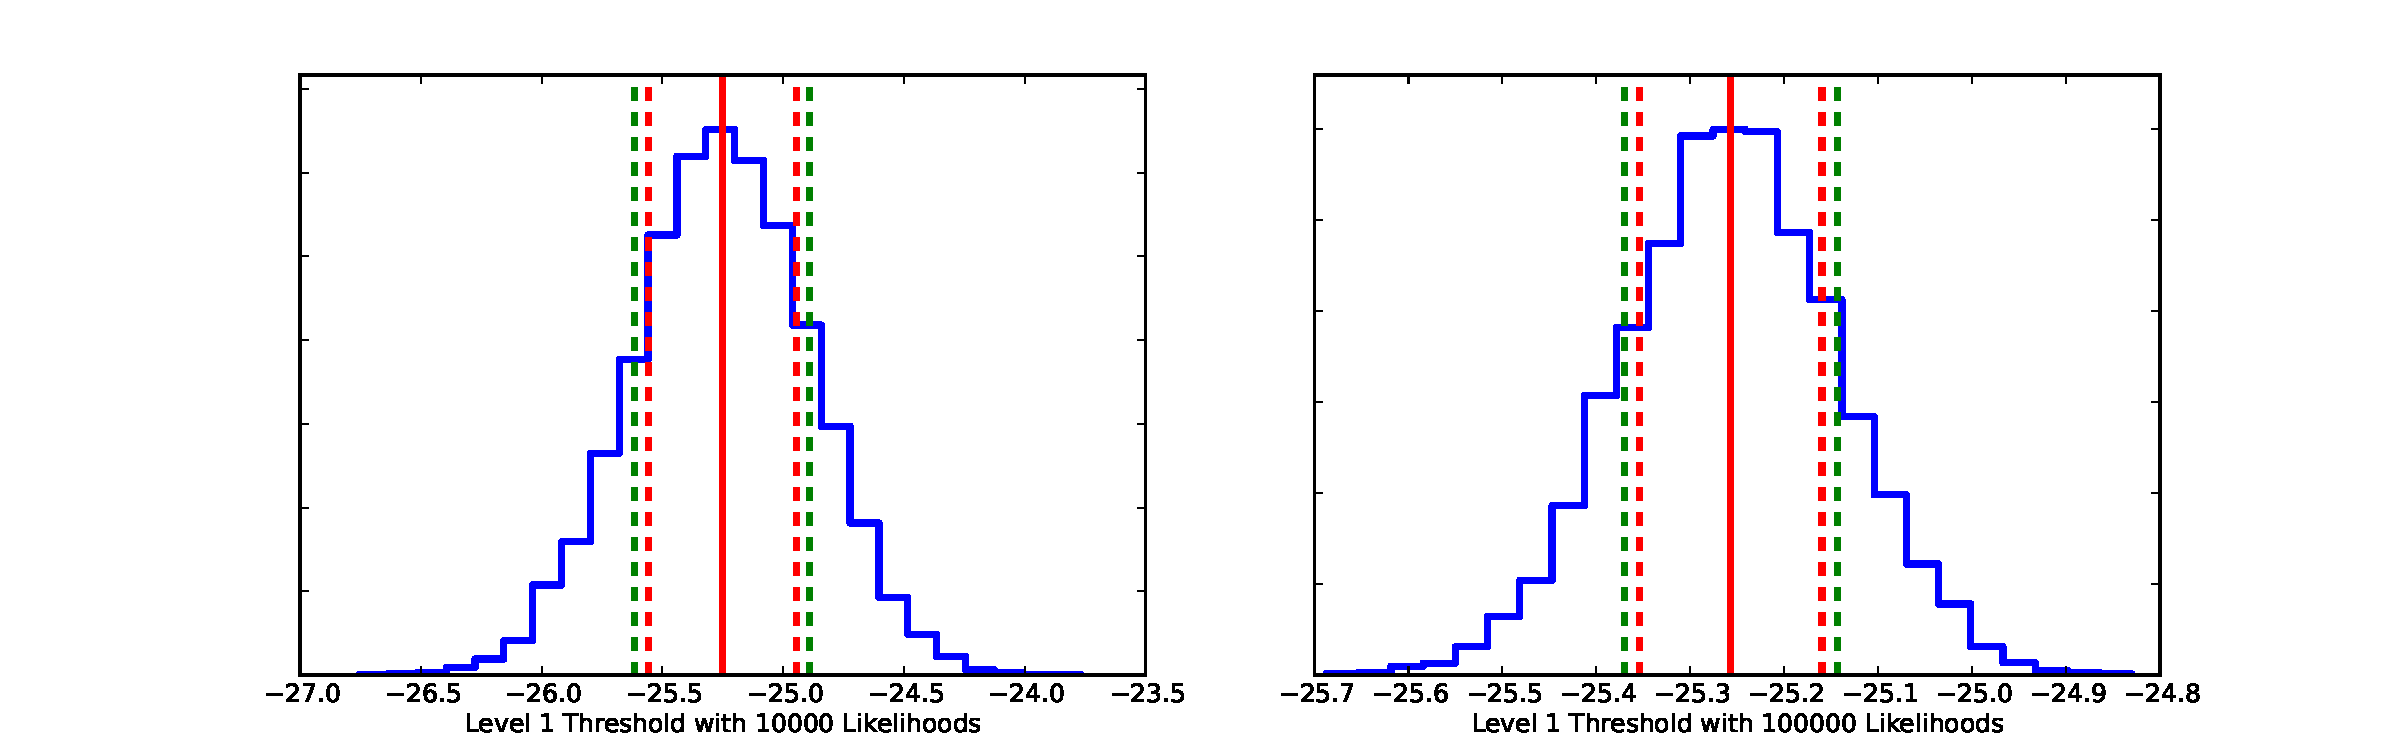
\includegraphics[width=0.99\linewidth]{level1.pdf}\\
 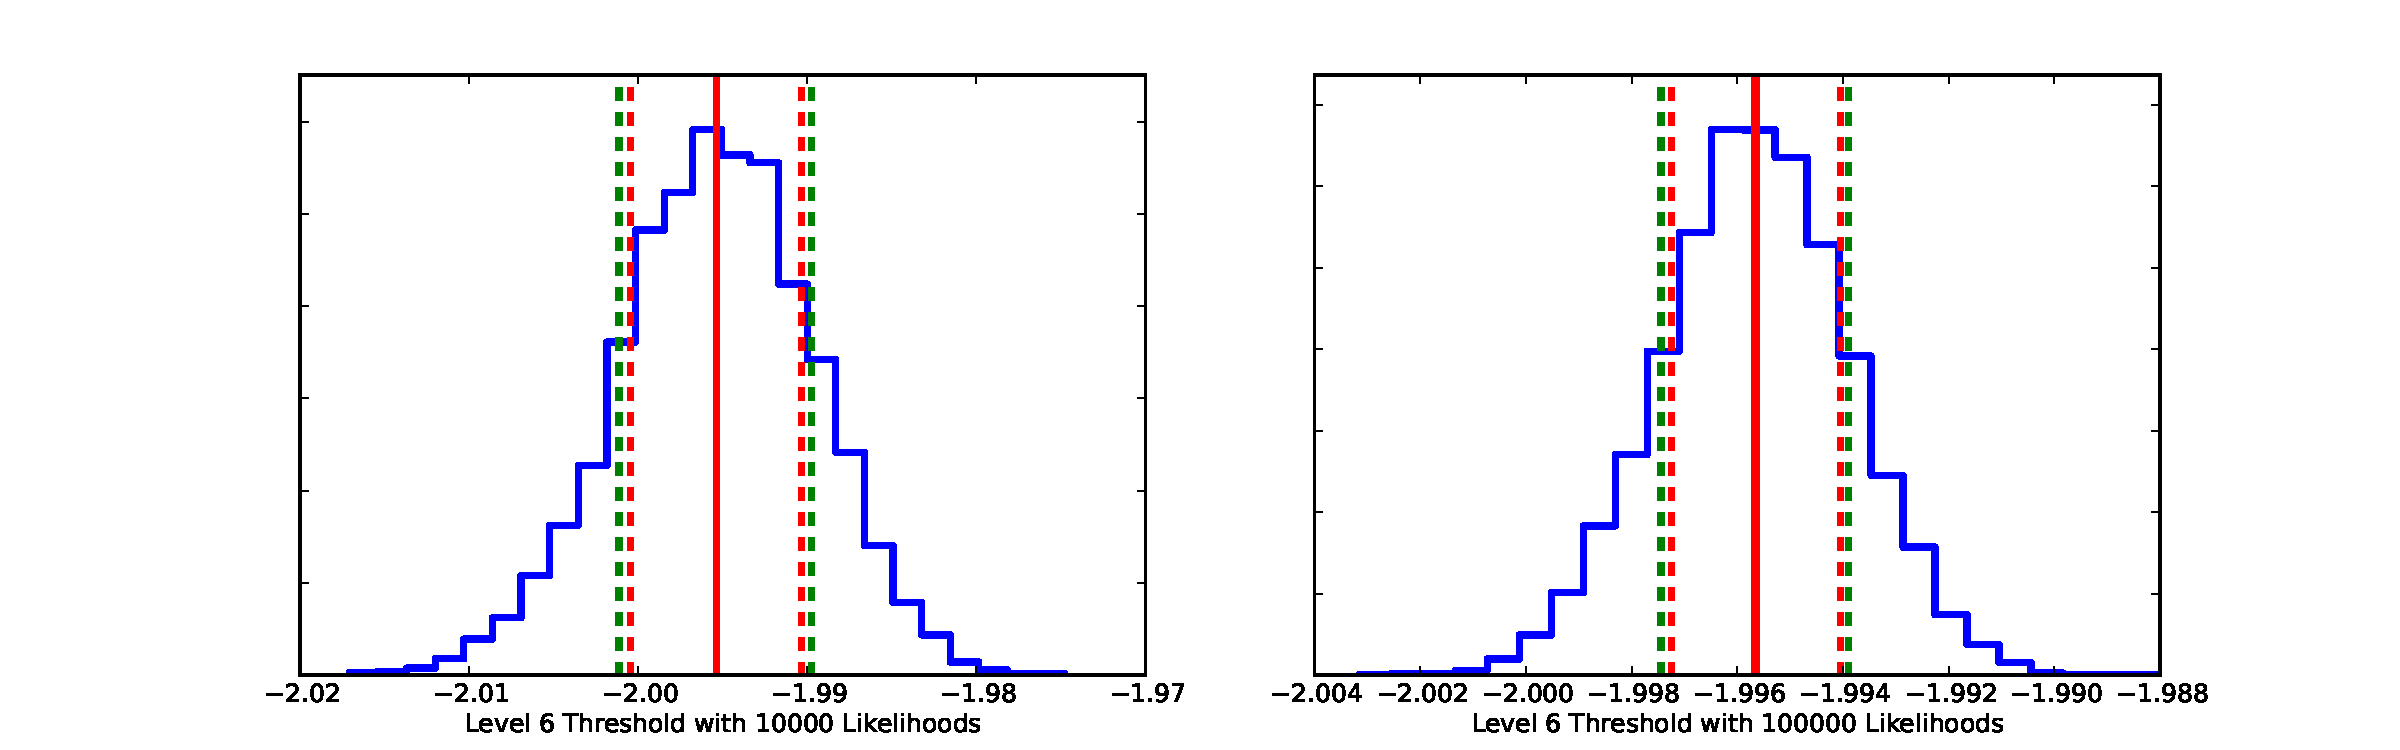
\includegraphics[width=0.99\linewidth]{level6.pdf}
 \caption{Level 1 (upper) and Level 6 (lower): Both histograms are plotted with 25 bins and 10,000 samples. (Here samples mean repetitions of the experiment, not the samples of likelihood to build every single level.) The left-hand side is the histogram of levels built with $N_{1a}$ likelihoods and the right-hand side is the histogram of levels built with $N_{1b}$ likelihoods. The \textcolor{red}{red} solid lines indicate the true values of the logarithm of the likelihood thresholds of levels and \textcolor{darkgreen}{dark green} solid lines indicate the experimental mean of the logarithm of the likelihood thresholds, which cannot be distinguished from the true values in these pictures. The \textcolor{red}{red} dashed lines indicate the theoretical standard deviation and the \textcolor{darkgreen}{dark green} dashed lines indicate the experimental standard deviation.}
 \label{fig:level1-6}
\end{figure}

\begin{figure}[h]
 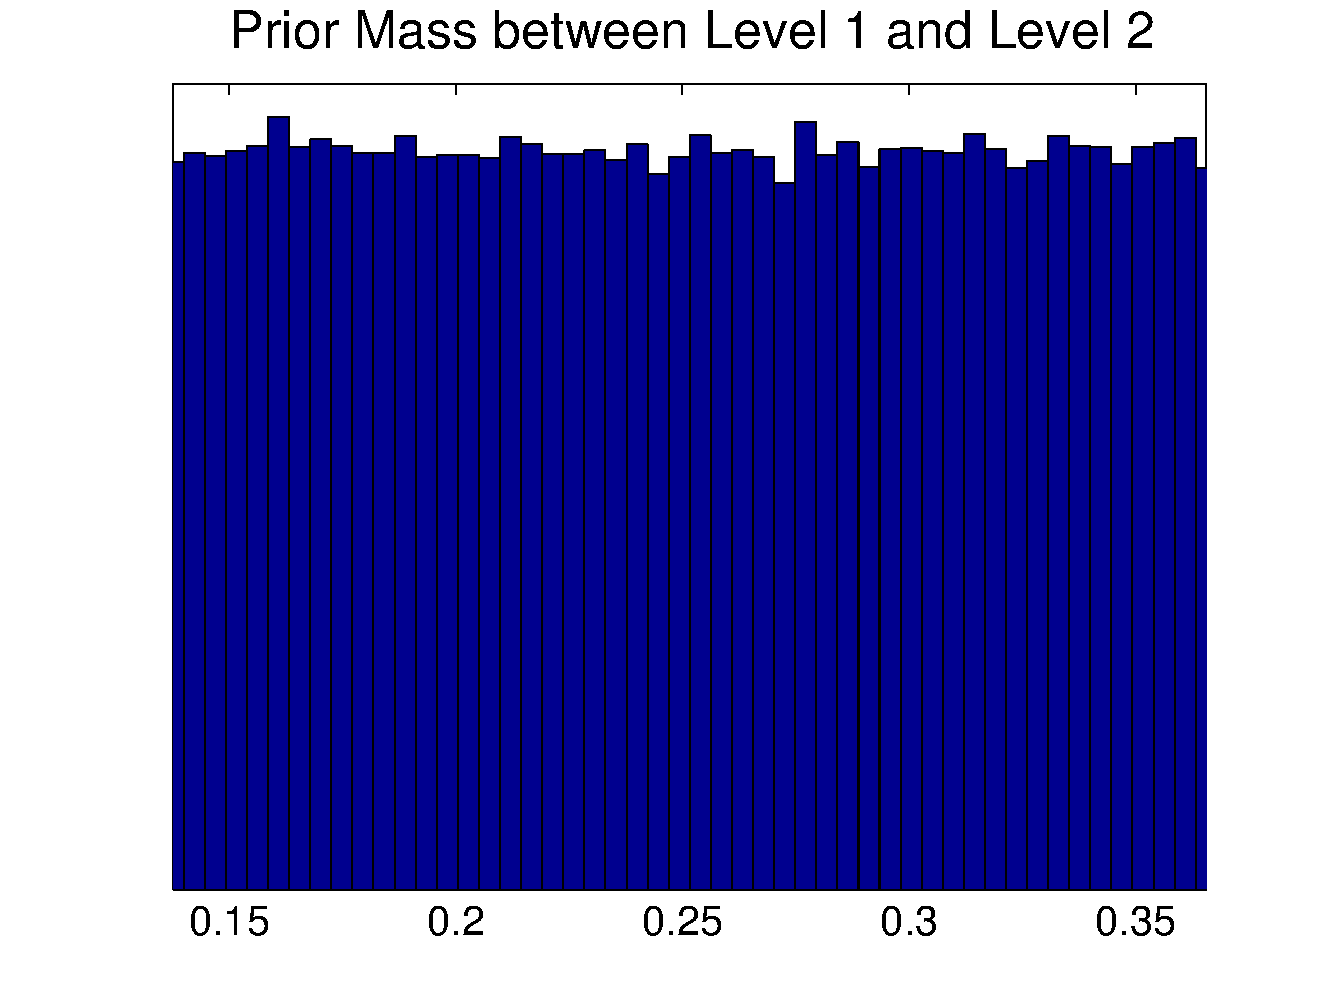
\includegraphics[width=0.45\linewidth]{histgaps-01-02.pdf}
 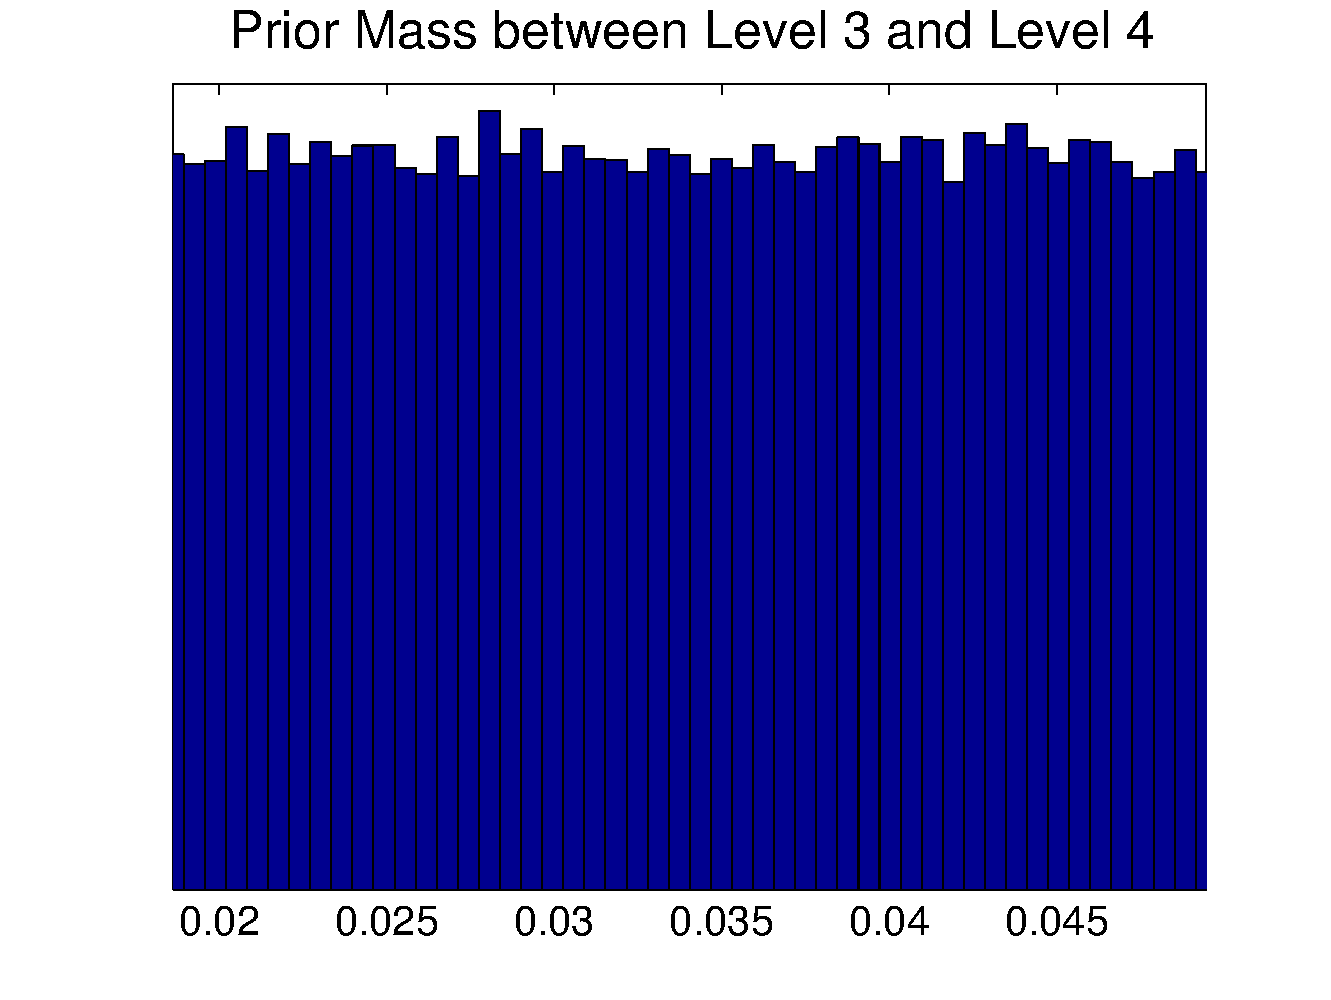
\includegraphics[width=0.45\linewidth]{histgaps-03-04.pdf}\\
 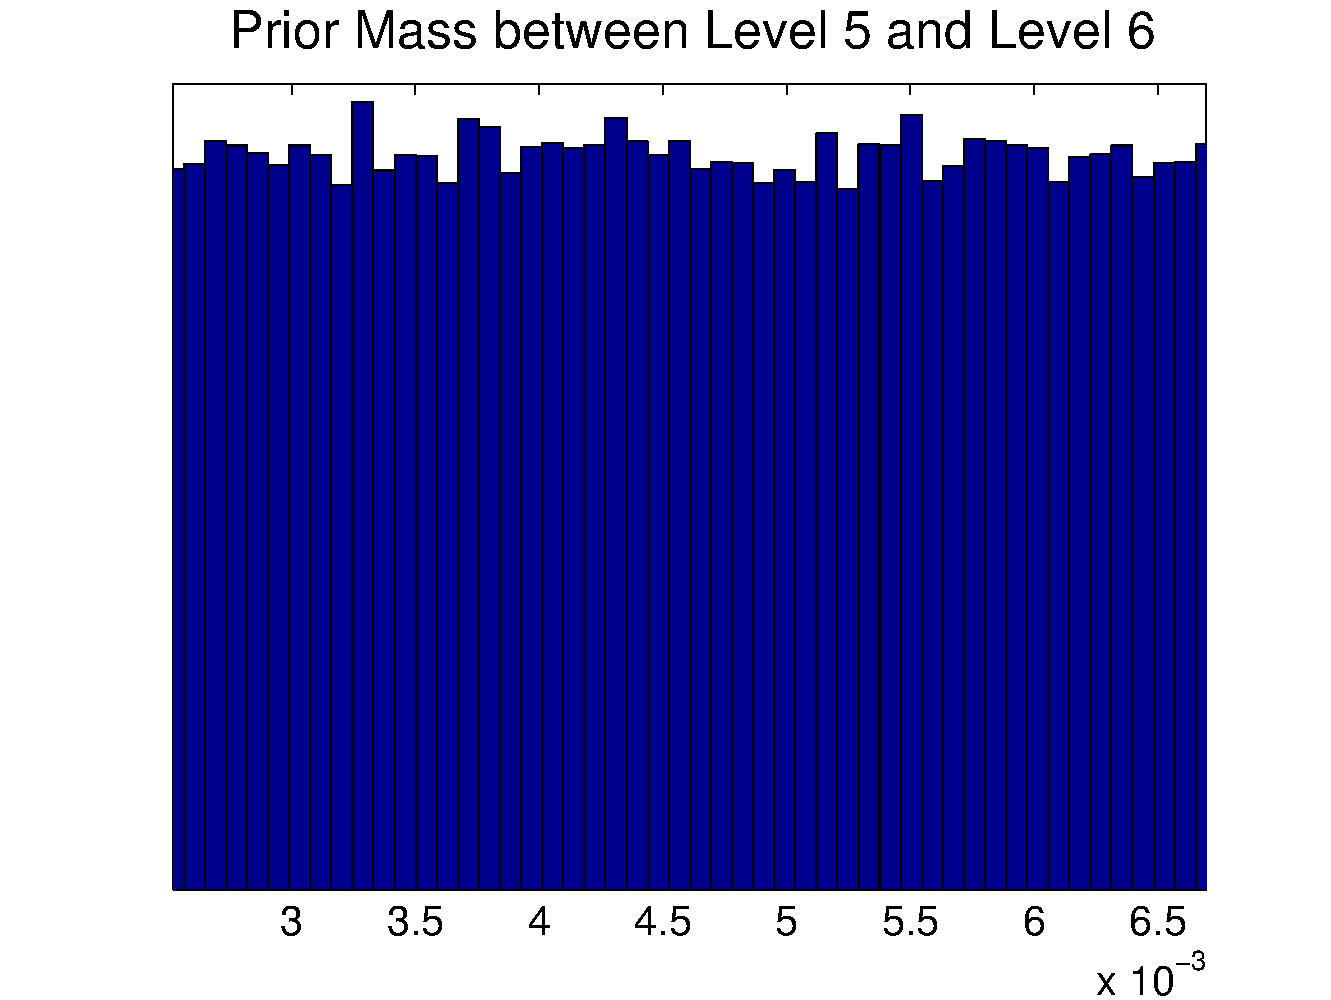
\includegraphics[width=0.45\linewidth]{histgaps-05-06.pdf}
 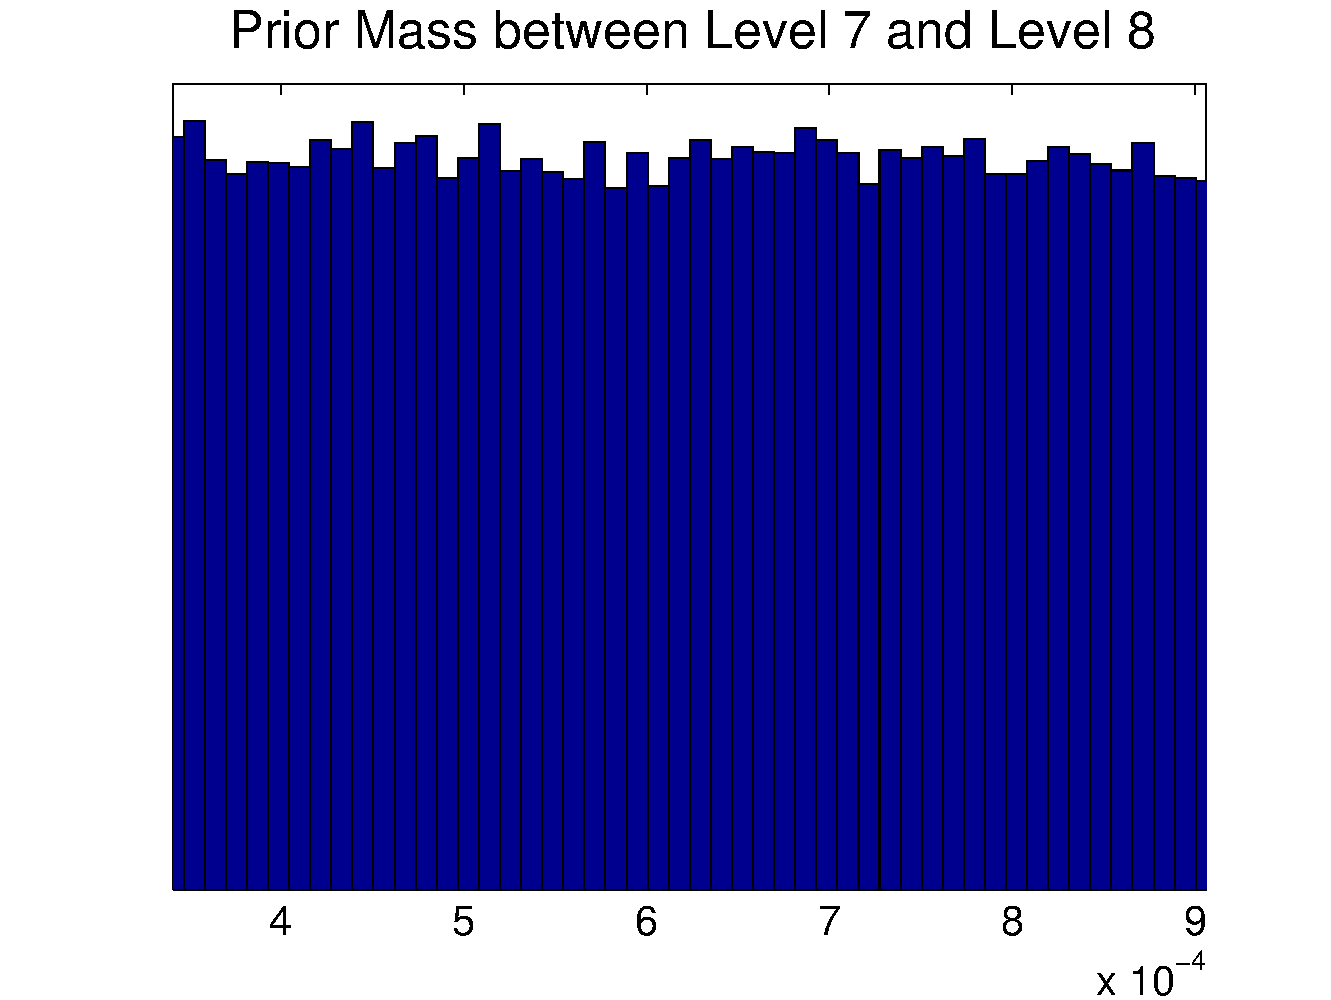
\includegraphics[width=0.45\linewidth]{histgaps-07-08.pdf} \\
\caption{Histograms of prior masses of samples inside a bin sandwiched by two adjacent levels. 4 examples are given. All are approximately uniform distribution.}
 \label{fig:hist-gaps}
\end{figure}

\begin{figure}[h]
 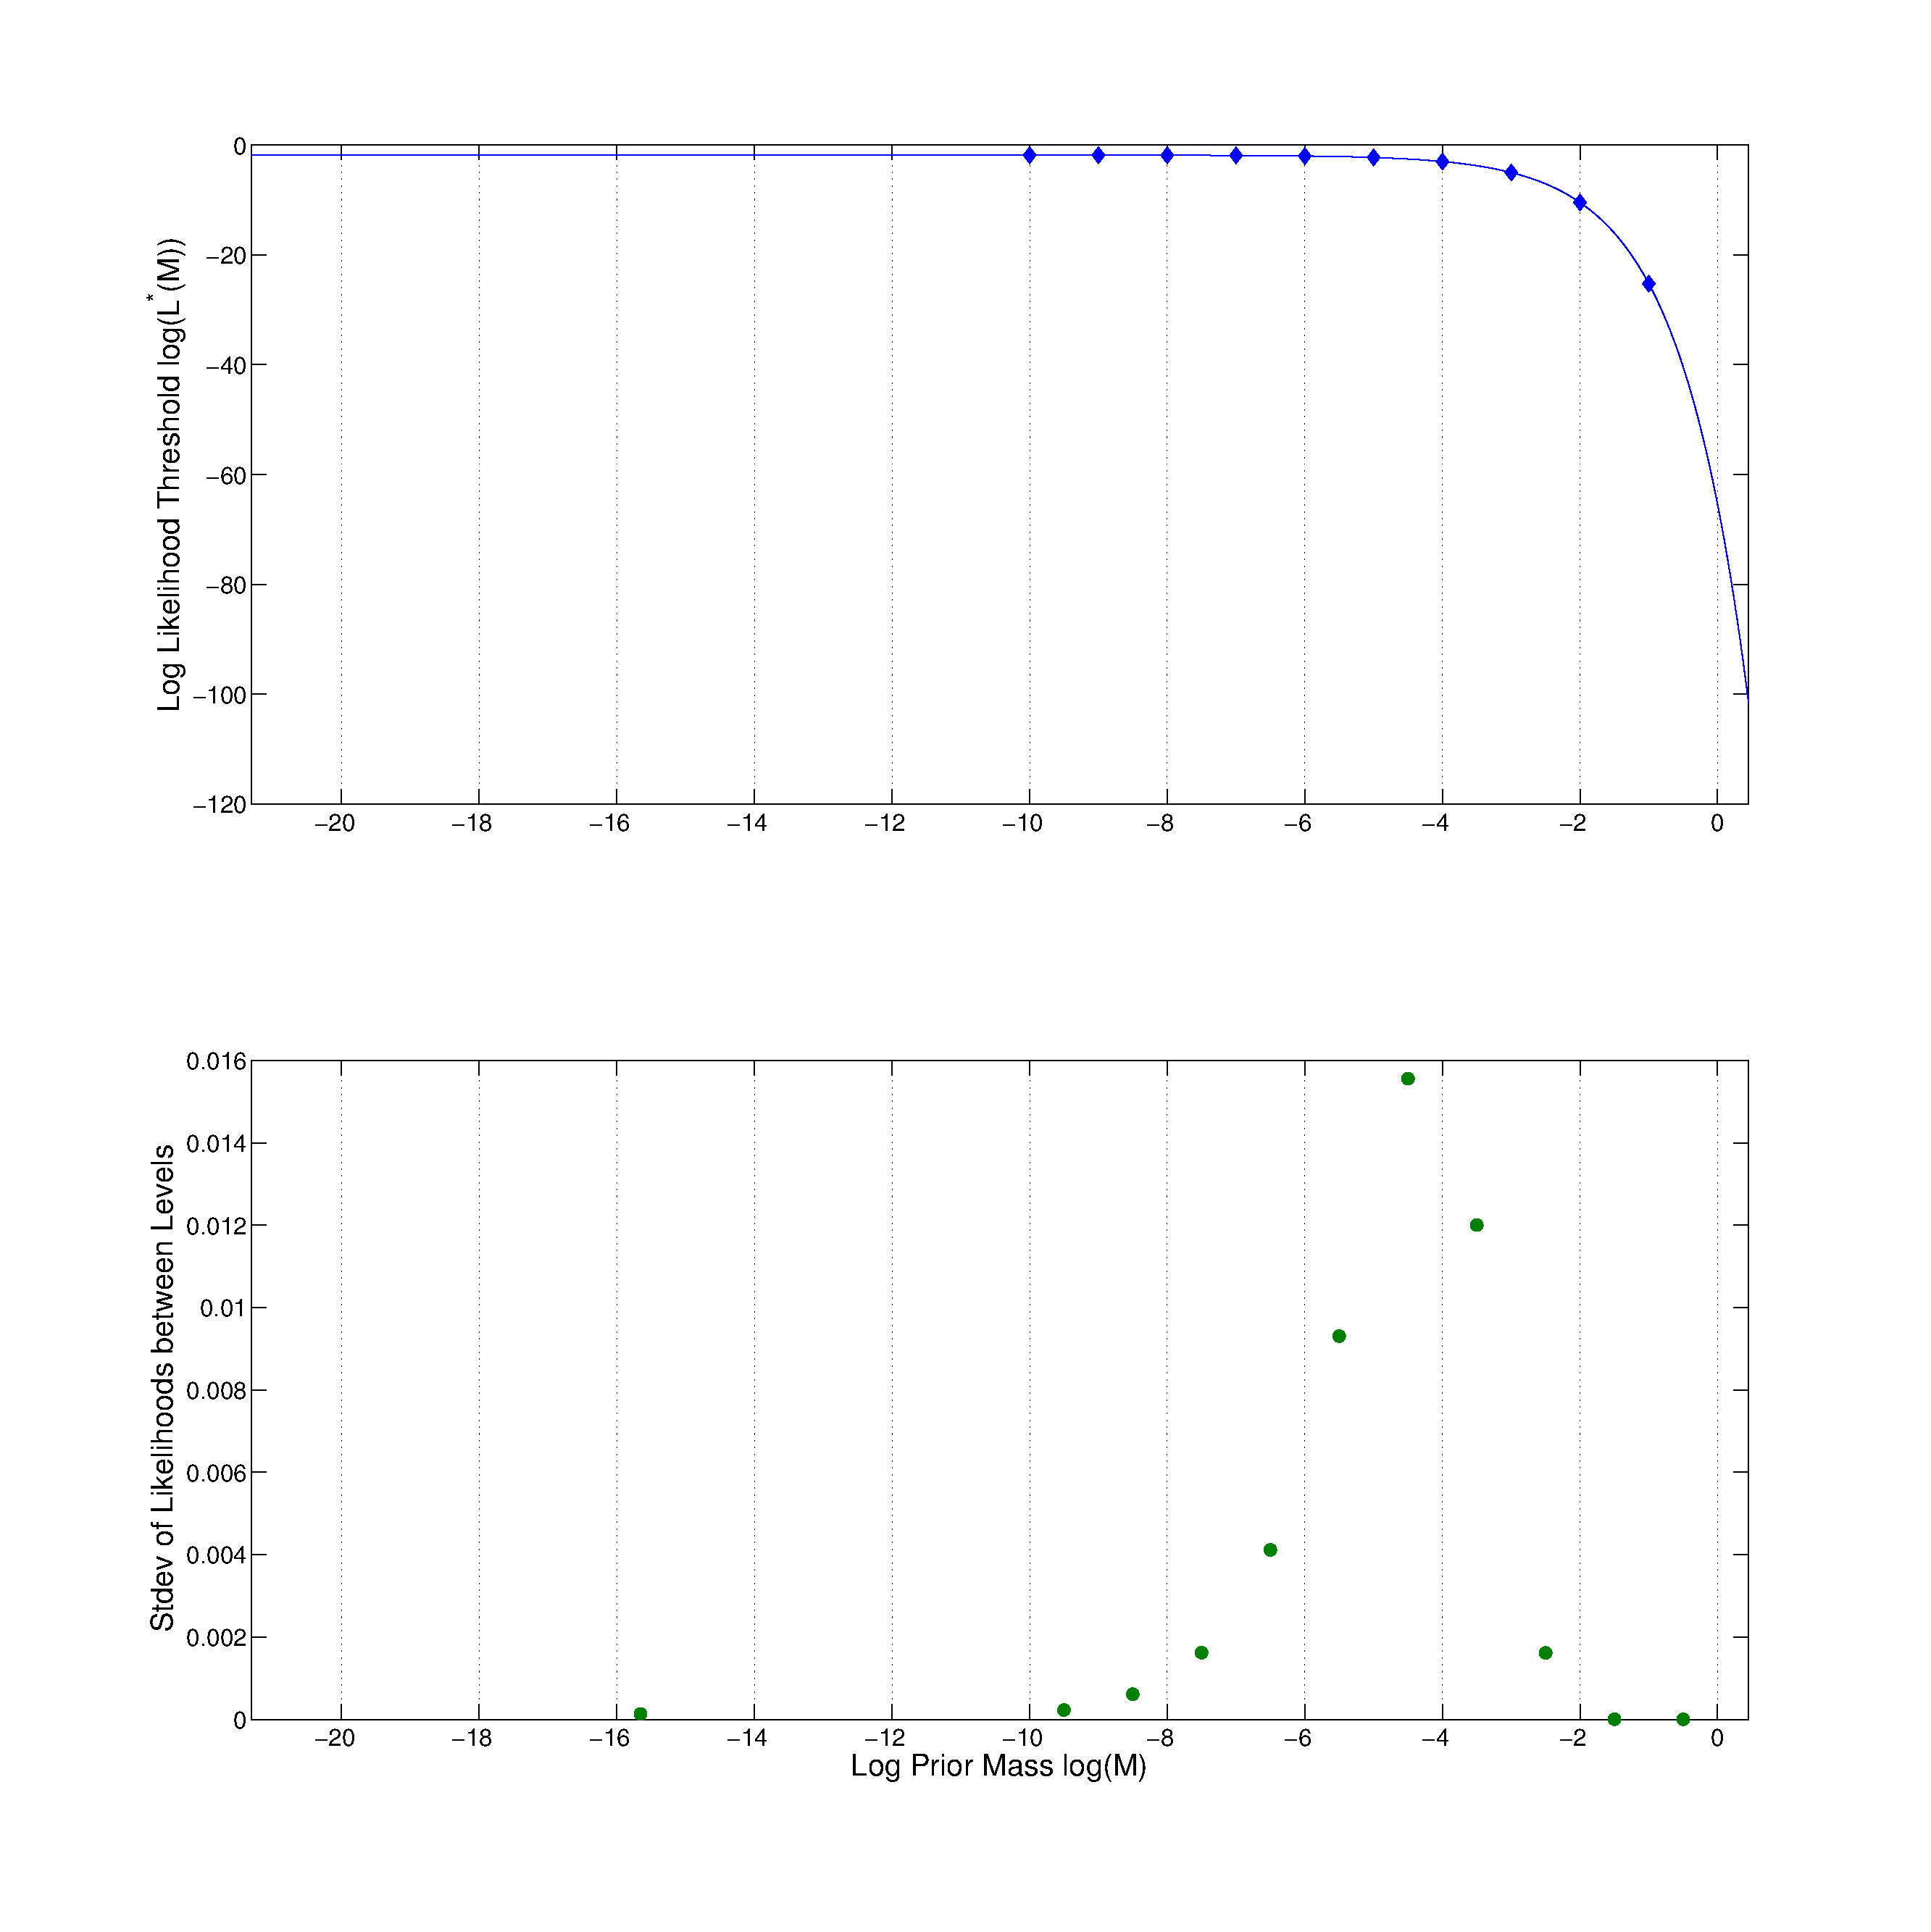
\includegraphics[width=0.99\linewidth]{stdev-between-gaps.pdf}
\caption{The 10 levels in the figure are the true levels summarized in Tab. (\ref{tab:true-levels}). Notice that the standard deviation of likelihood samples between level 3 ($\log{M} = -3$) and level 6 ($\log{M} = -6$) will pretty much determine the standard deviation of the final result.}
 \label{fig:level-var}
\end{figure}

\begin{table}[h]
\centering
std for 10-d case ($\times10^{-15}$)\\
\begin{tabular}{c|c|c|c}
\hline
 & $N_1=10^4$ & $N_1=3\times10^4$ & $N_1=10^5$\\
\hline
$N_2=10^6$                  & 3.1760  & 3.2465 & 3.1653 \\
$N_2=3\times10^6$ & 1.8297  & 1.8816 & 1.8390 \\
$N_2=10^7$                  & 0.9887  & 0.9704 &  1.0238\\
\hline
\end{tabular}
\caption{The standard deviations for different $N_1$'s and $N_2$'s. The experiments are repeated for $1,000$ times. Compared with evidence value $9.77\times10^{-14}$, all the standard deviations are reasonably small. But $N_2$ is clearly more important in reducing variance. Note that there are 30 levels in this case, $30\times N_1$ and $N_2$ are actually comparable.}
\label{tab:N1N2}
\end{table} 

\begin{figure}
 \centering
 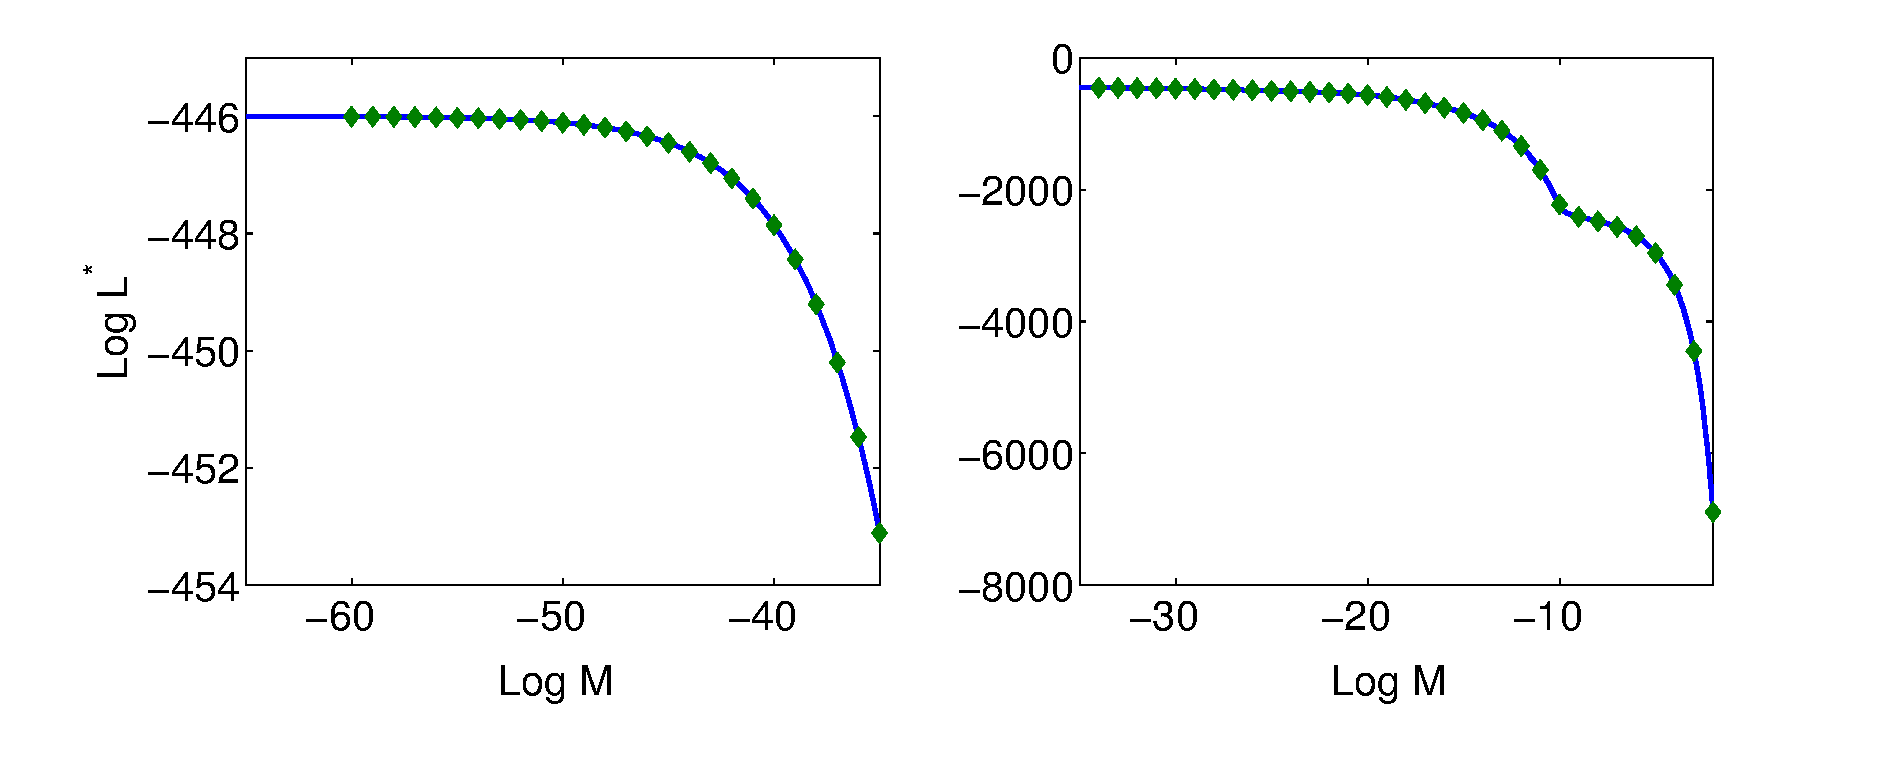
\includegraphics[width=0.99\linewidth]{Level_122_mod_1.pdf}\\
 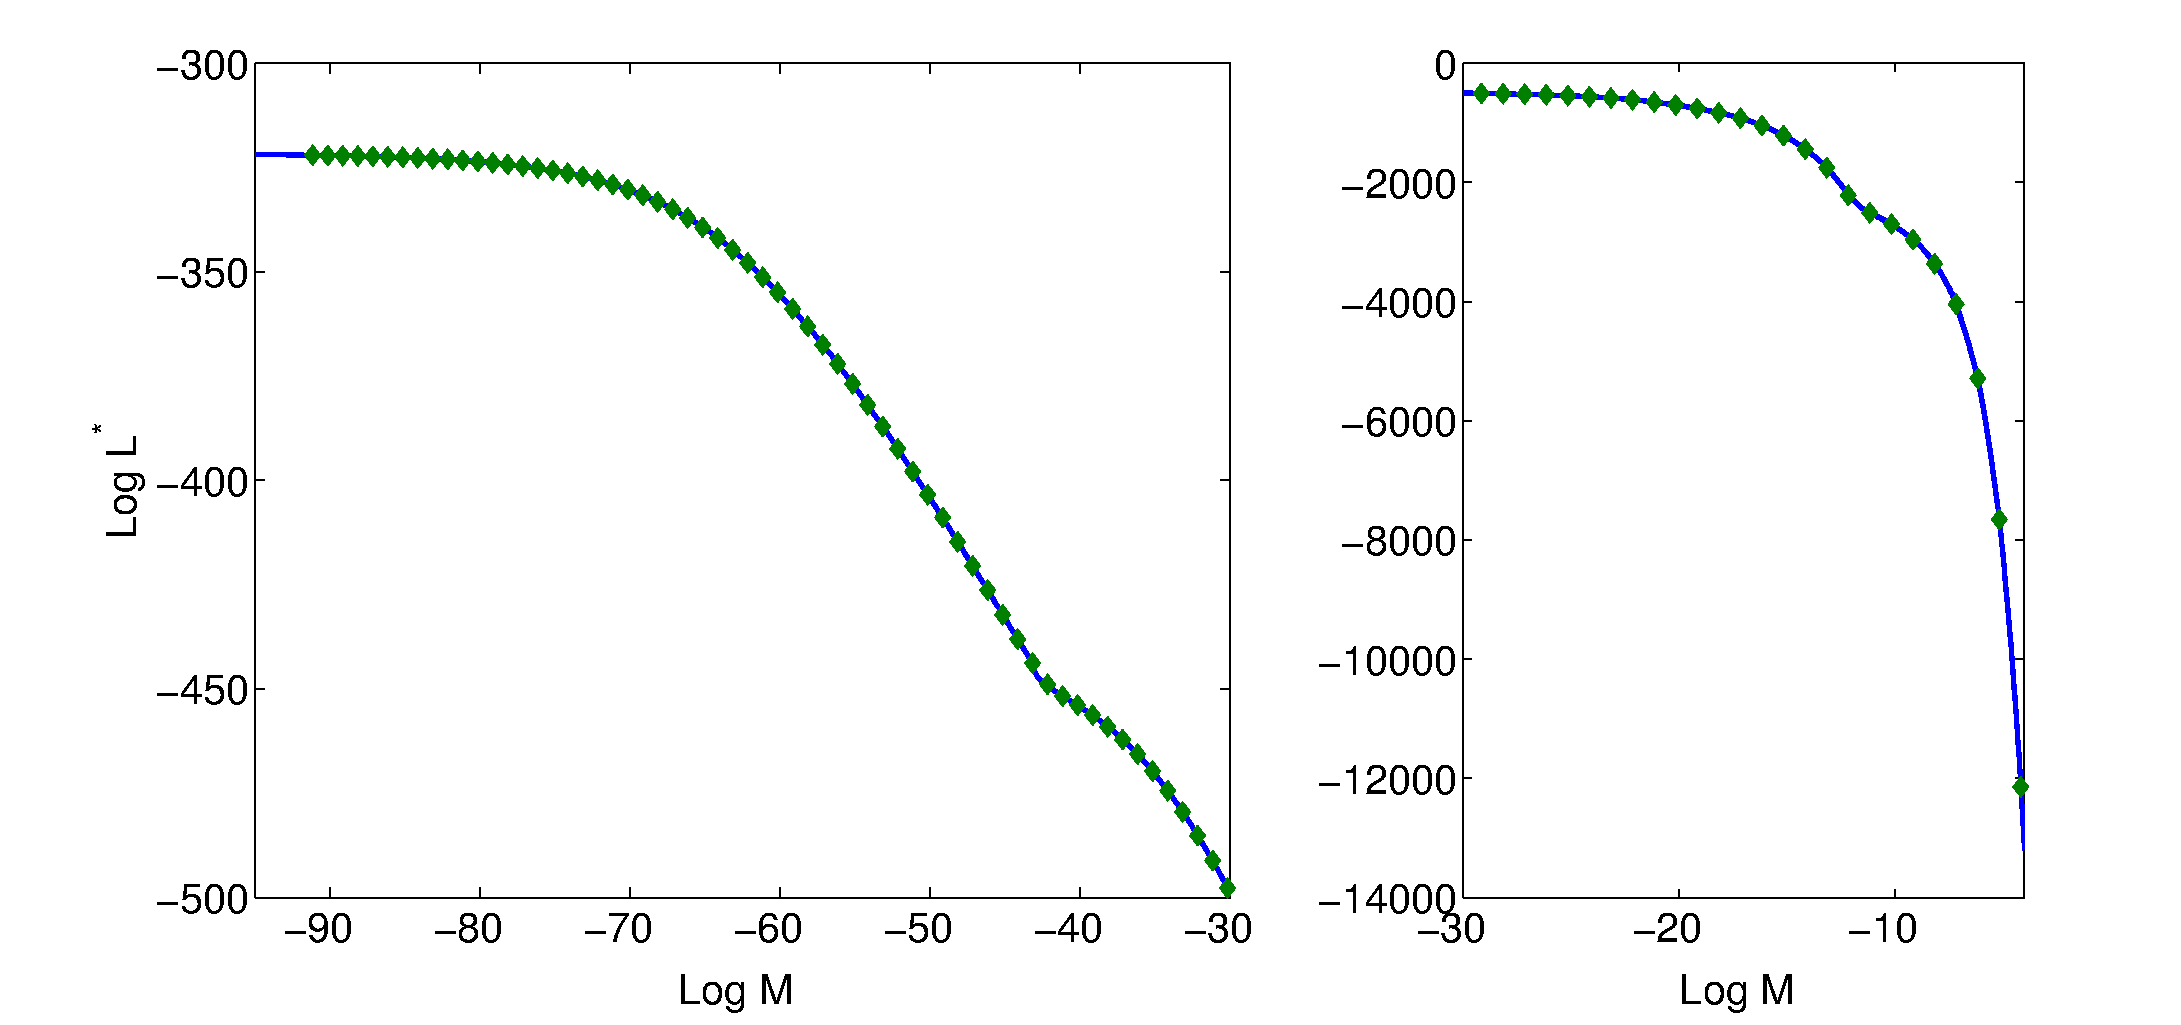
\includegraphics[width=0.9\linewidth]{Level_122_mod_2.pdf}\\
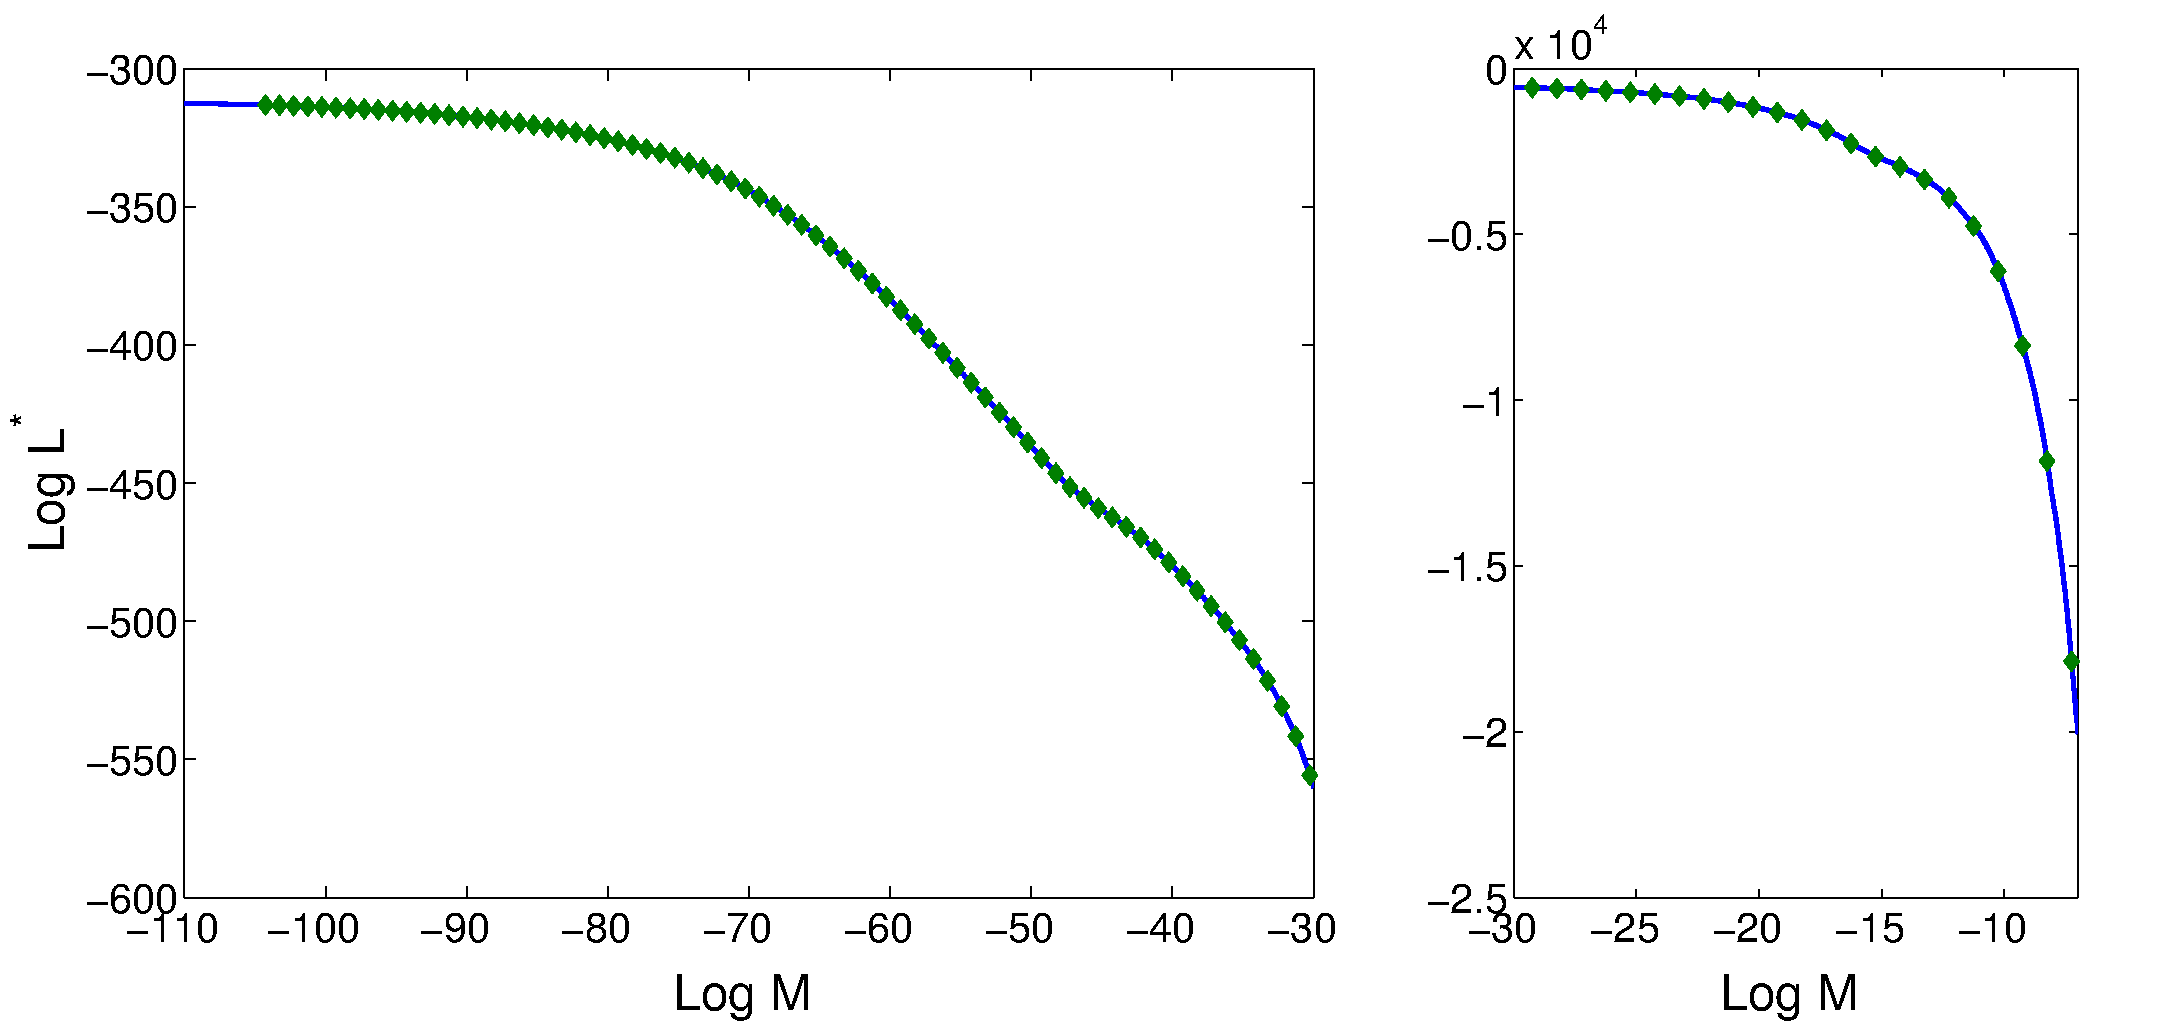
\includegraphics[width=0.9\linewidth]{Level_122_mod_3.pdf}
\caption{The 1st row shows the levels of 1-companion model. The 2nd row shows the levels of 2-companion model. The 3rd row shows the levels of 3-companion model.}
 \label{fig:levels-122}
\end{figure}

\begin{figure}
 \centering
 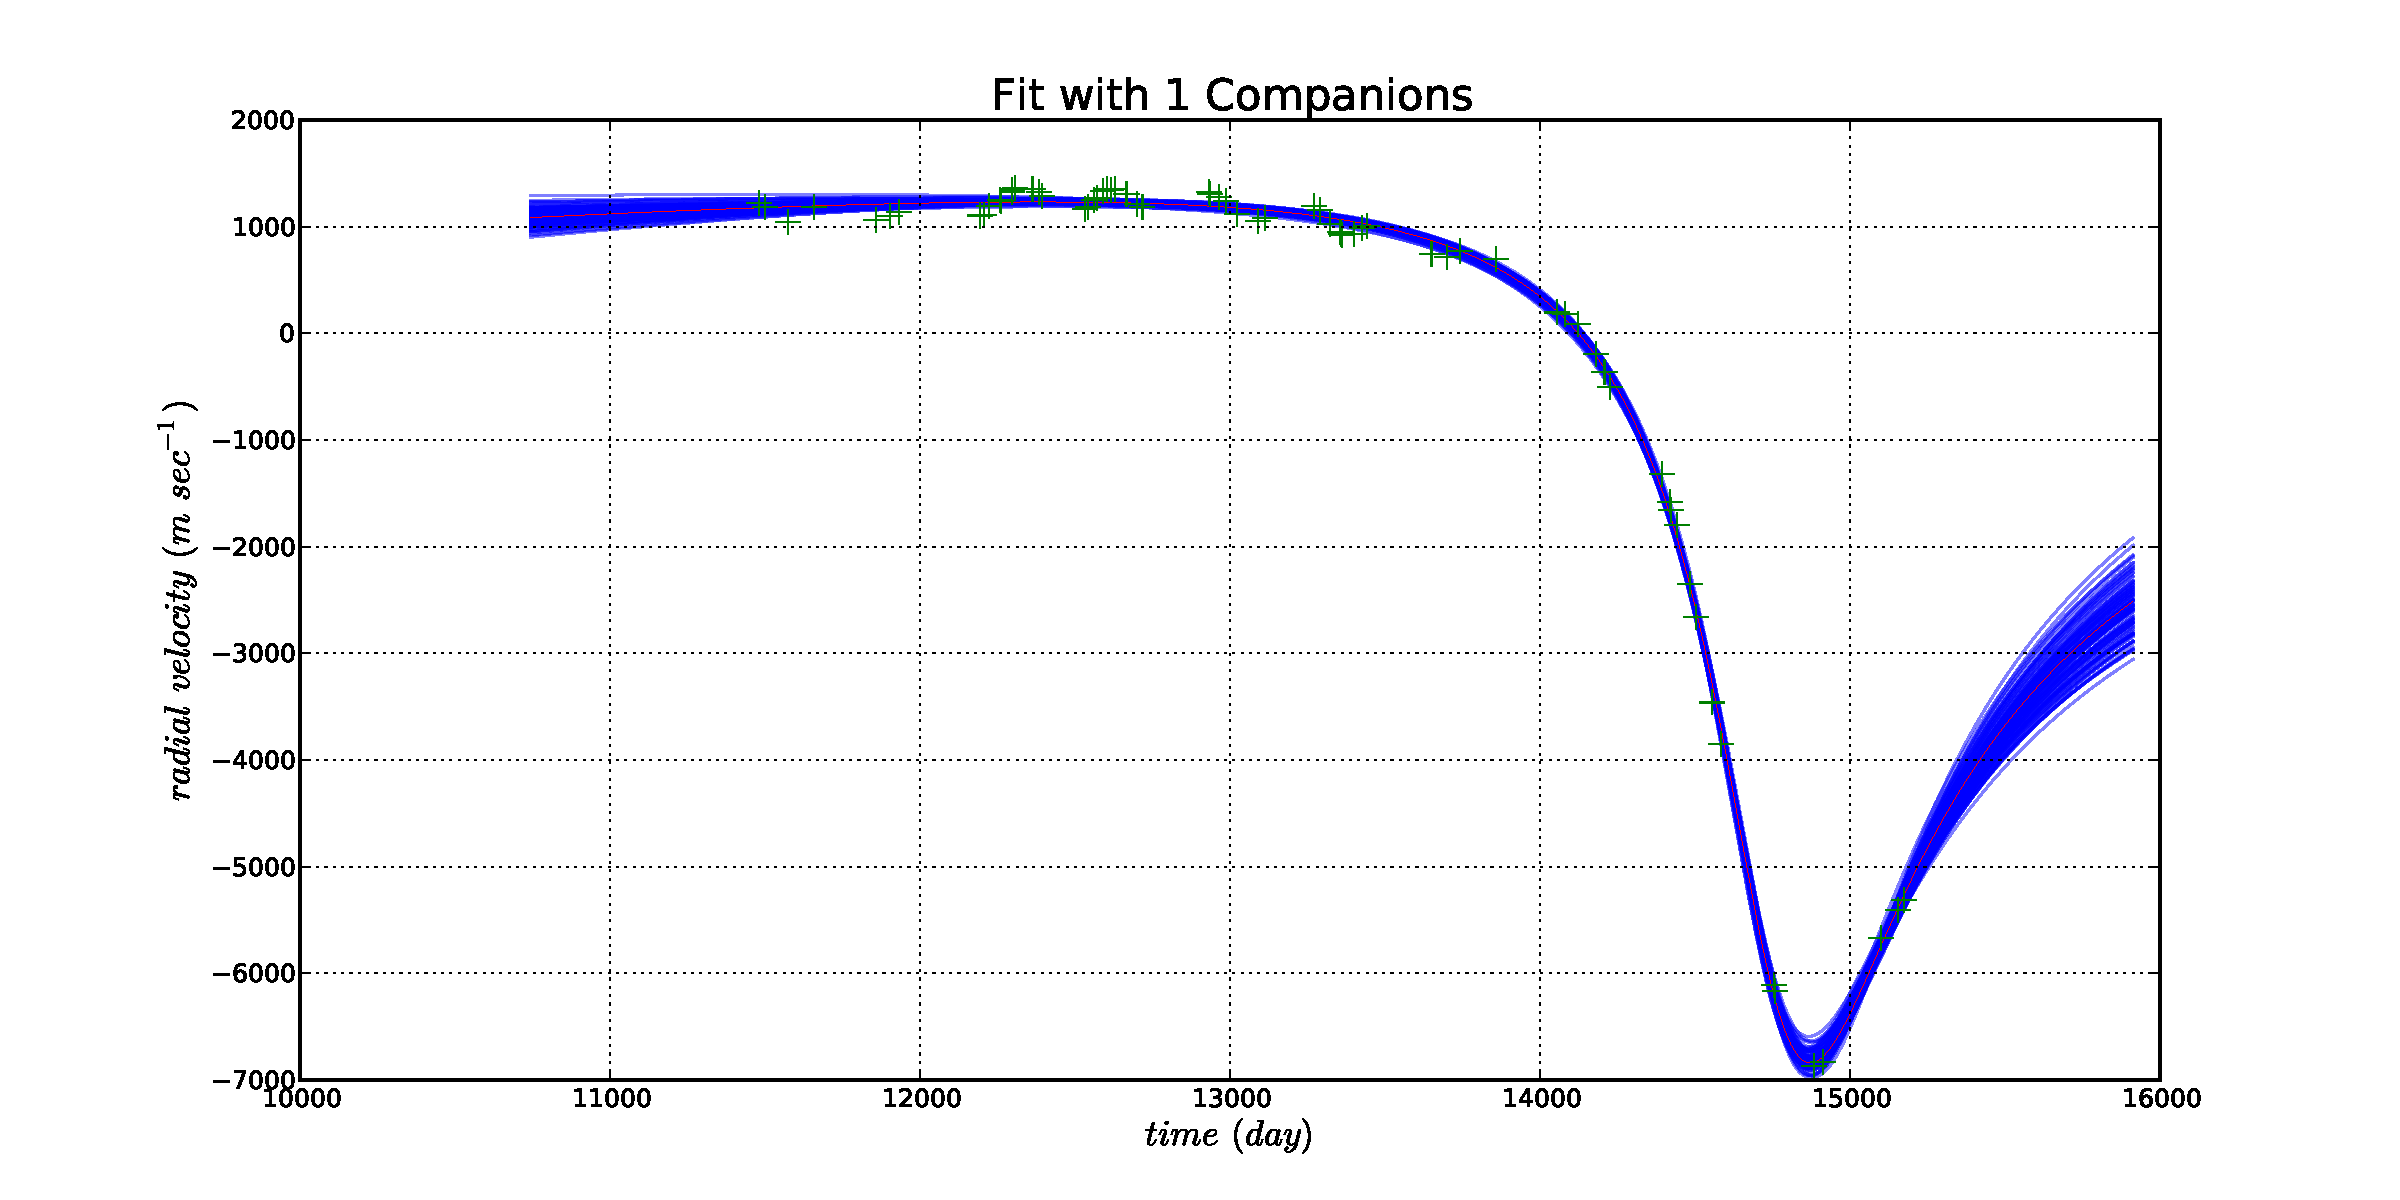
\includegraphics[width=0.85\linewidth]{fit_122_comp_1.pdf}\\
 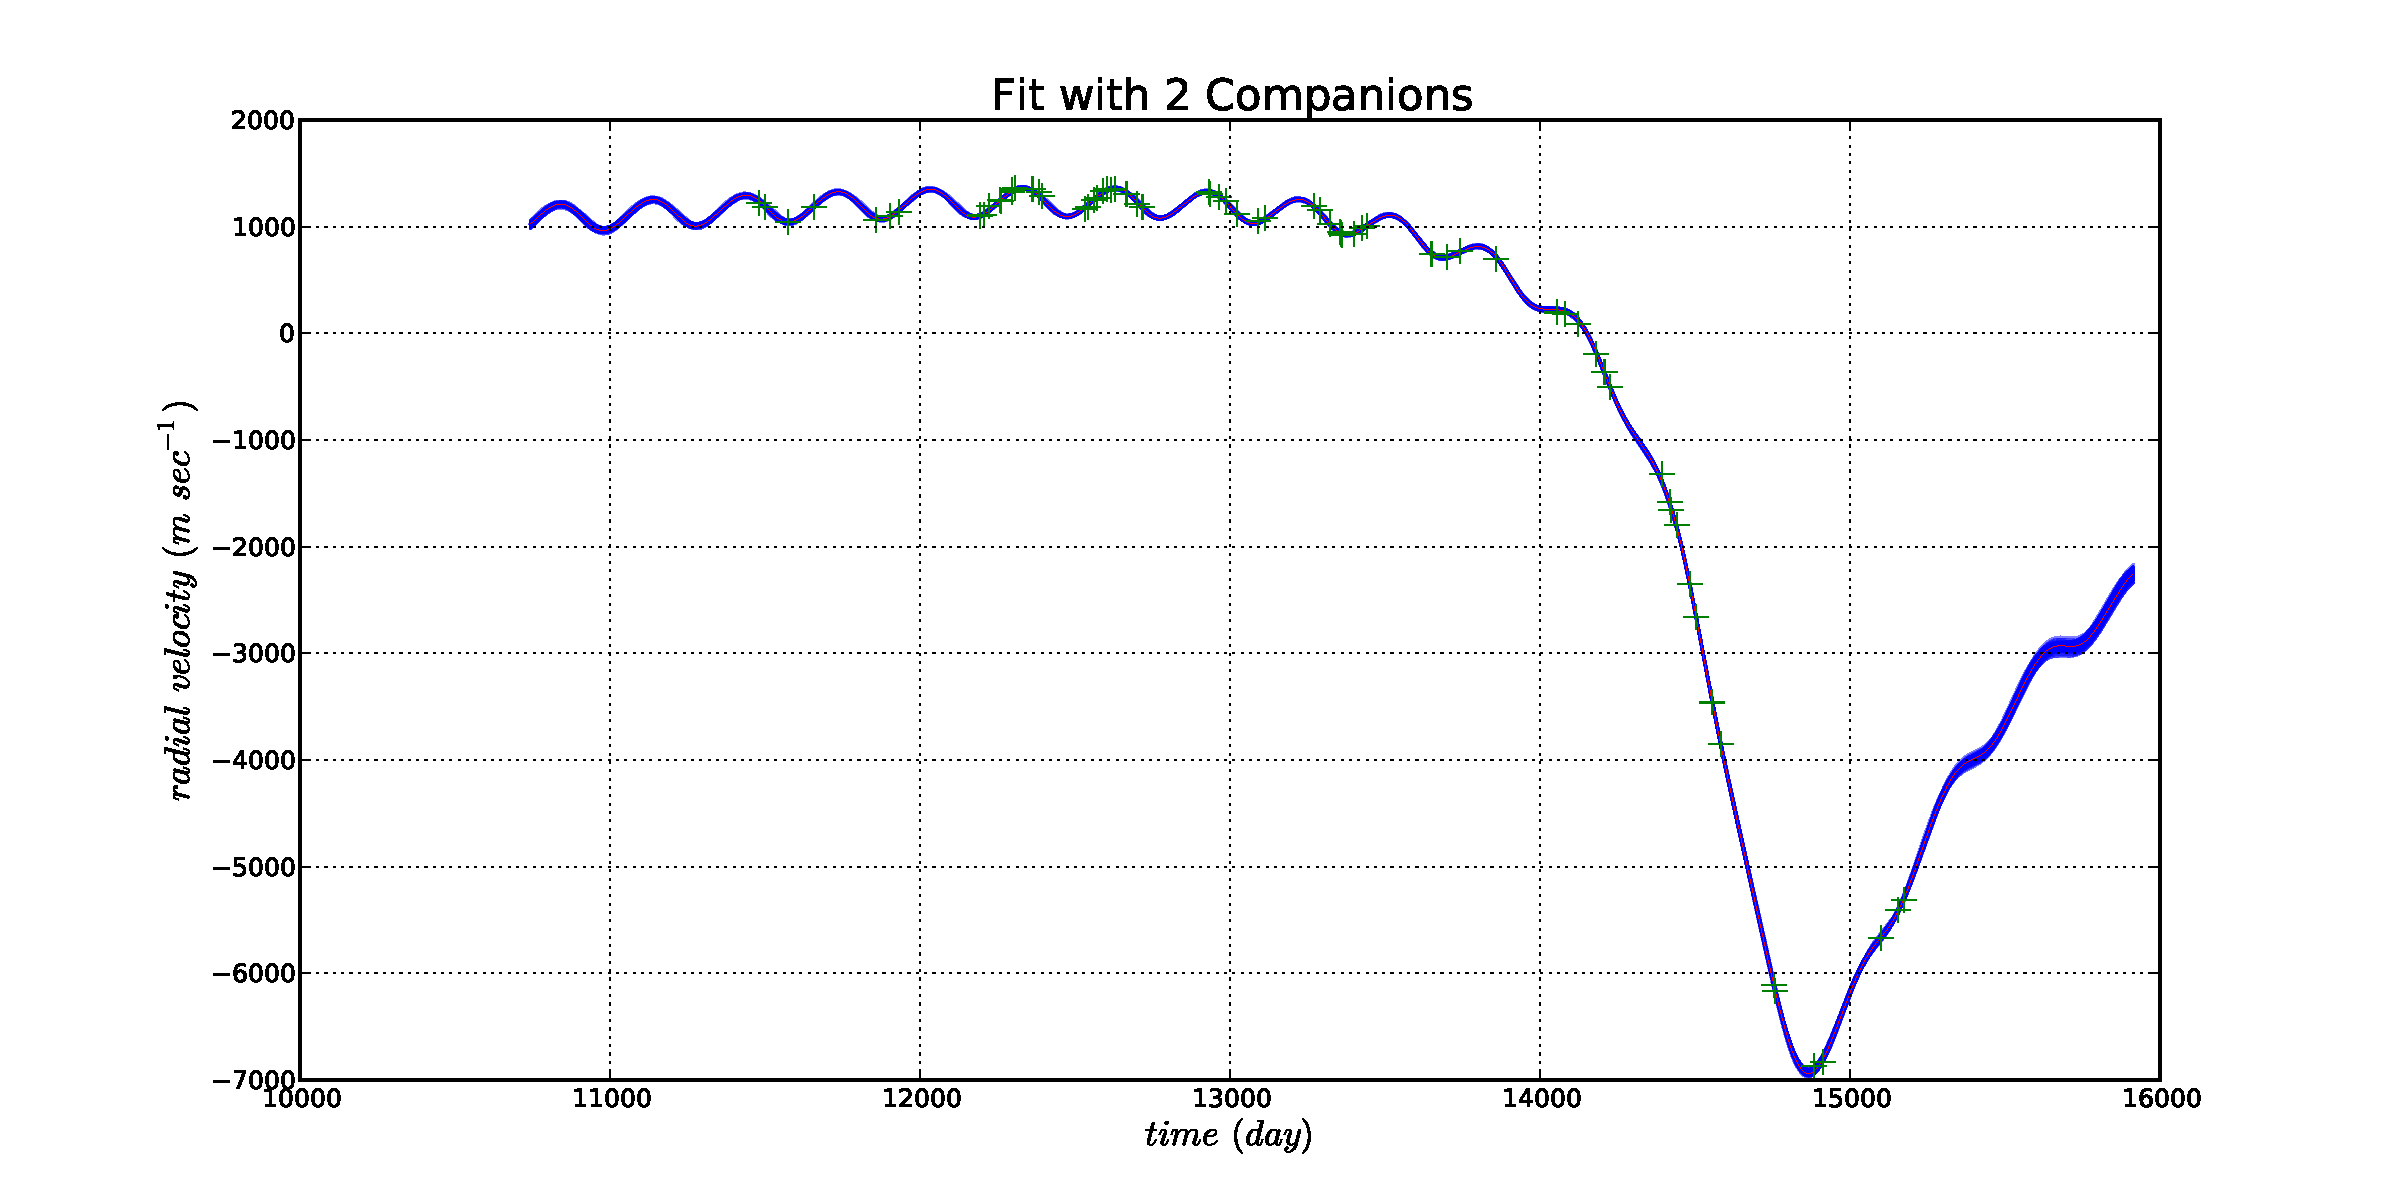
\includegraphics[width=0.85\linewidth]{fit_122_comp_2.pdf}\\
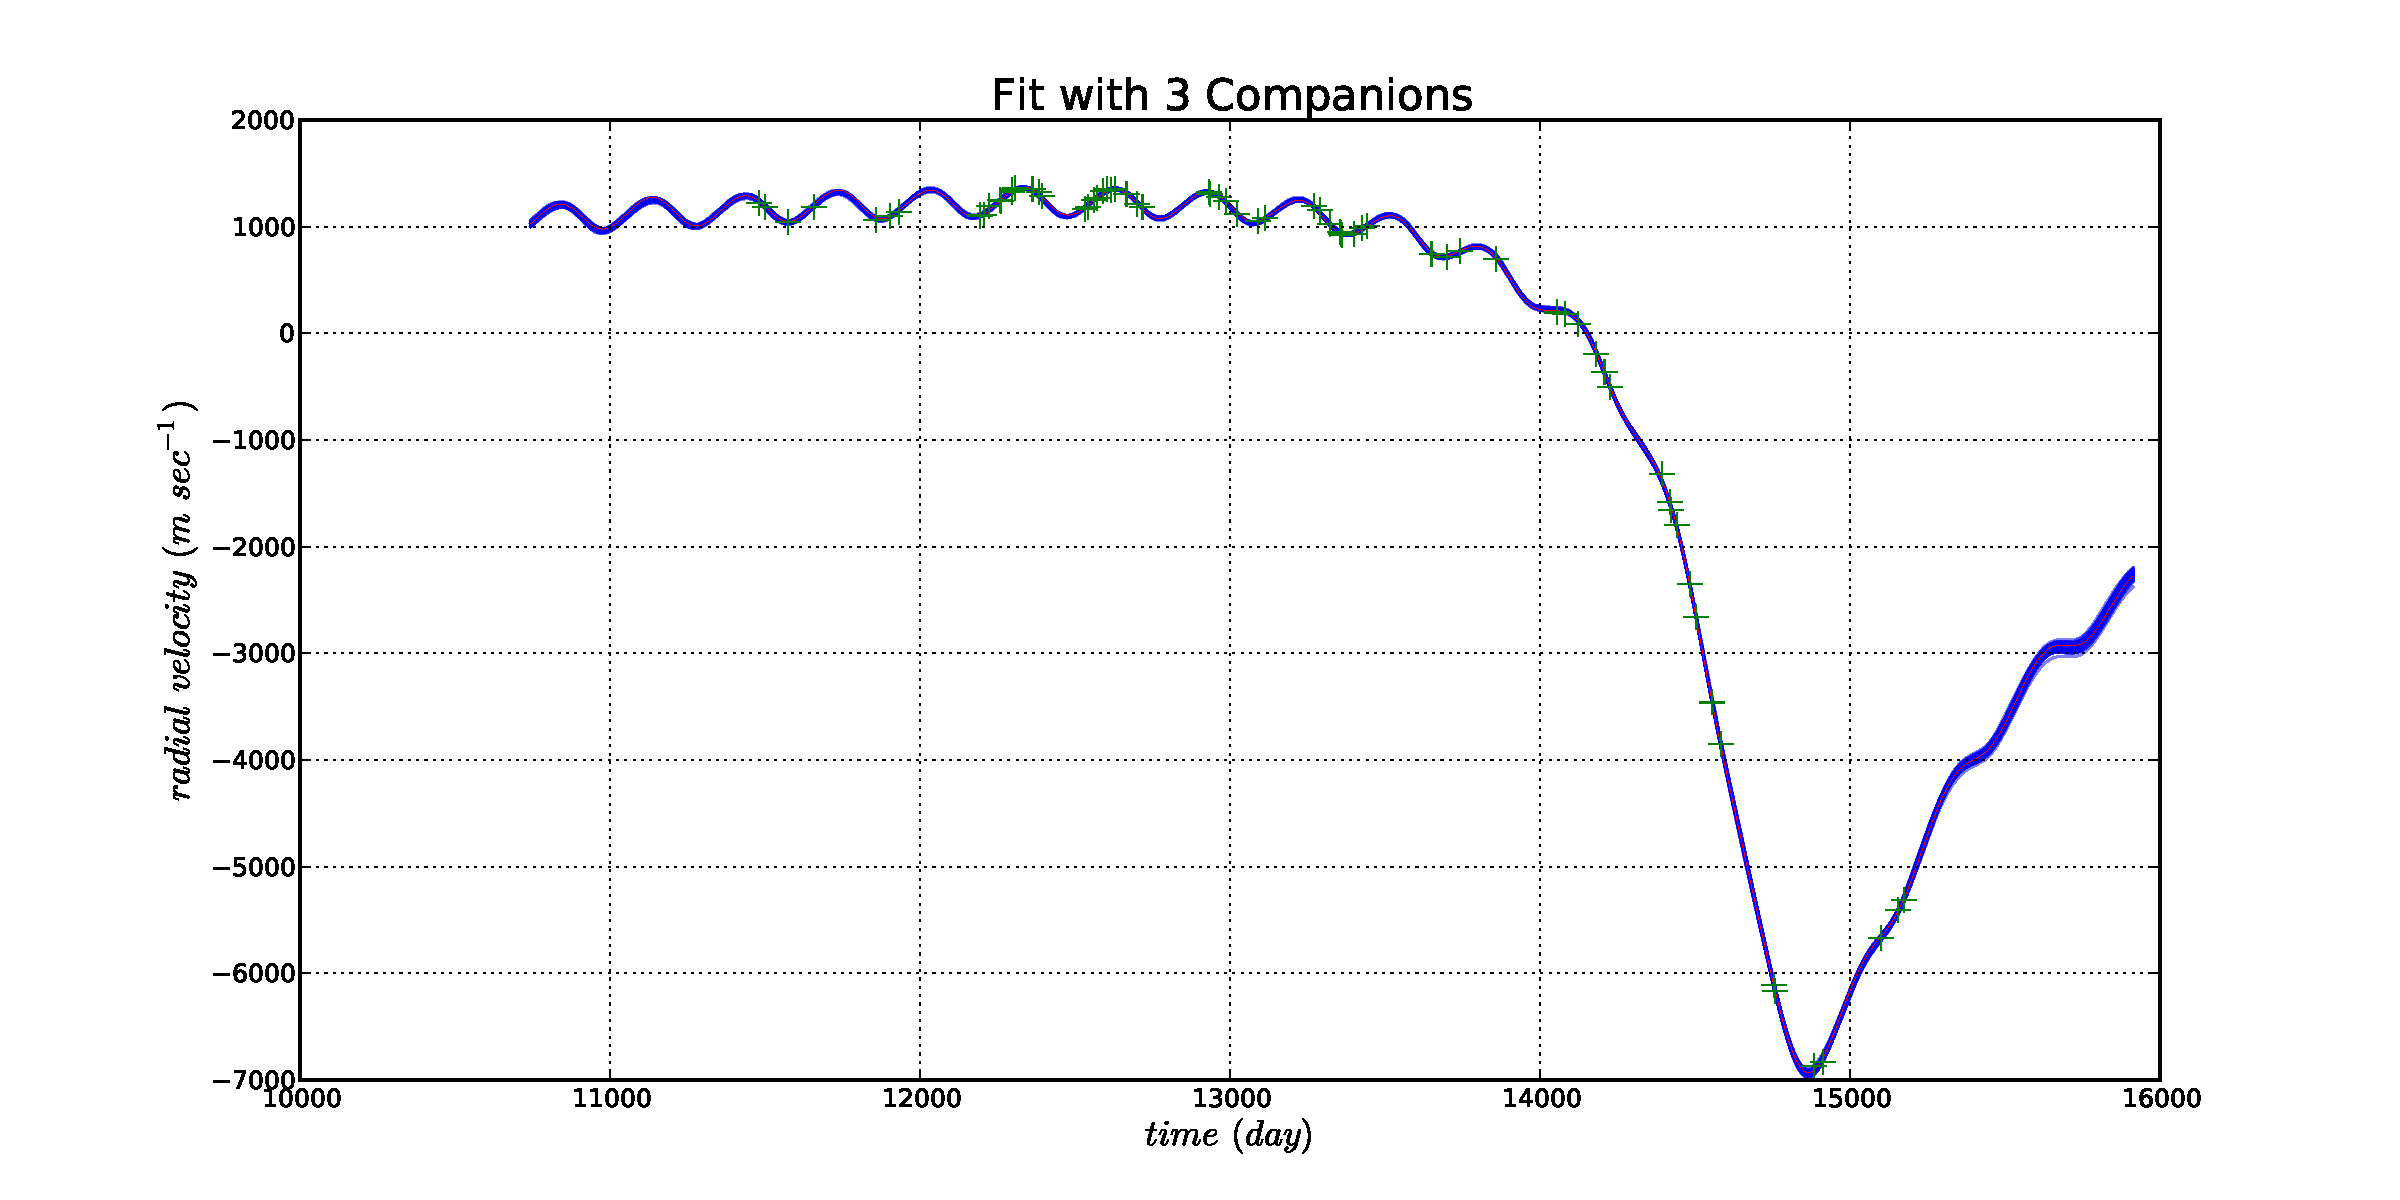
\includegraphics[width=0.85\linewidth]{fit_122_comp_3.pdf}
\caption{The 1st row shows the fit of 1-companion model. The 2nd row shows the fit of 2-companion model. The 3rd row shows the fit of 3-companion model. All the fits are drawn from the posterior of each model. The companion model is clearly not as good as the other two. The 2-companion and 3-companion models are not distinguishable from this view.}
 \label{fig:fit-122-1-2-3}
\end{figure}

\begin{figure}
 \centering
 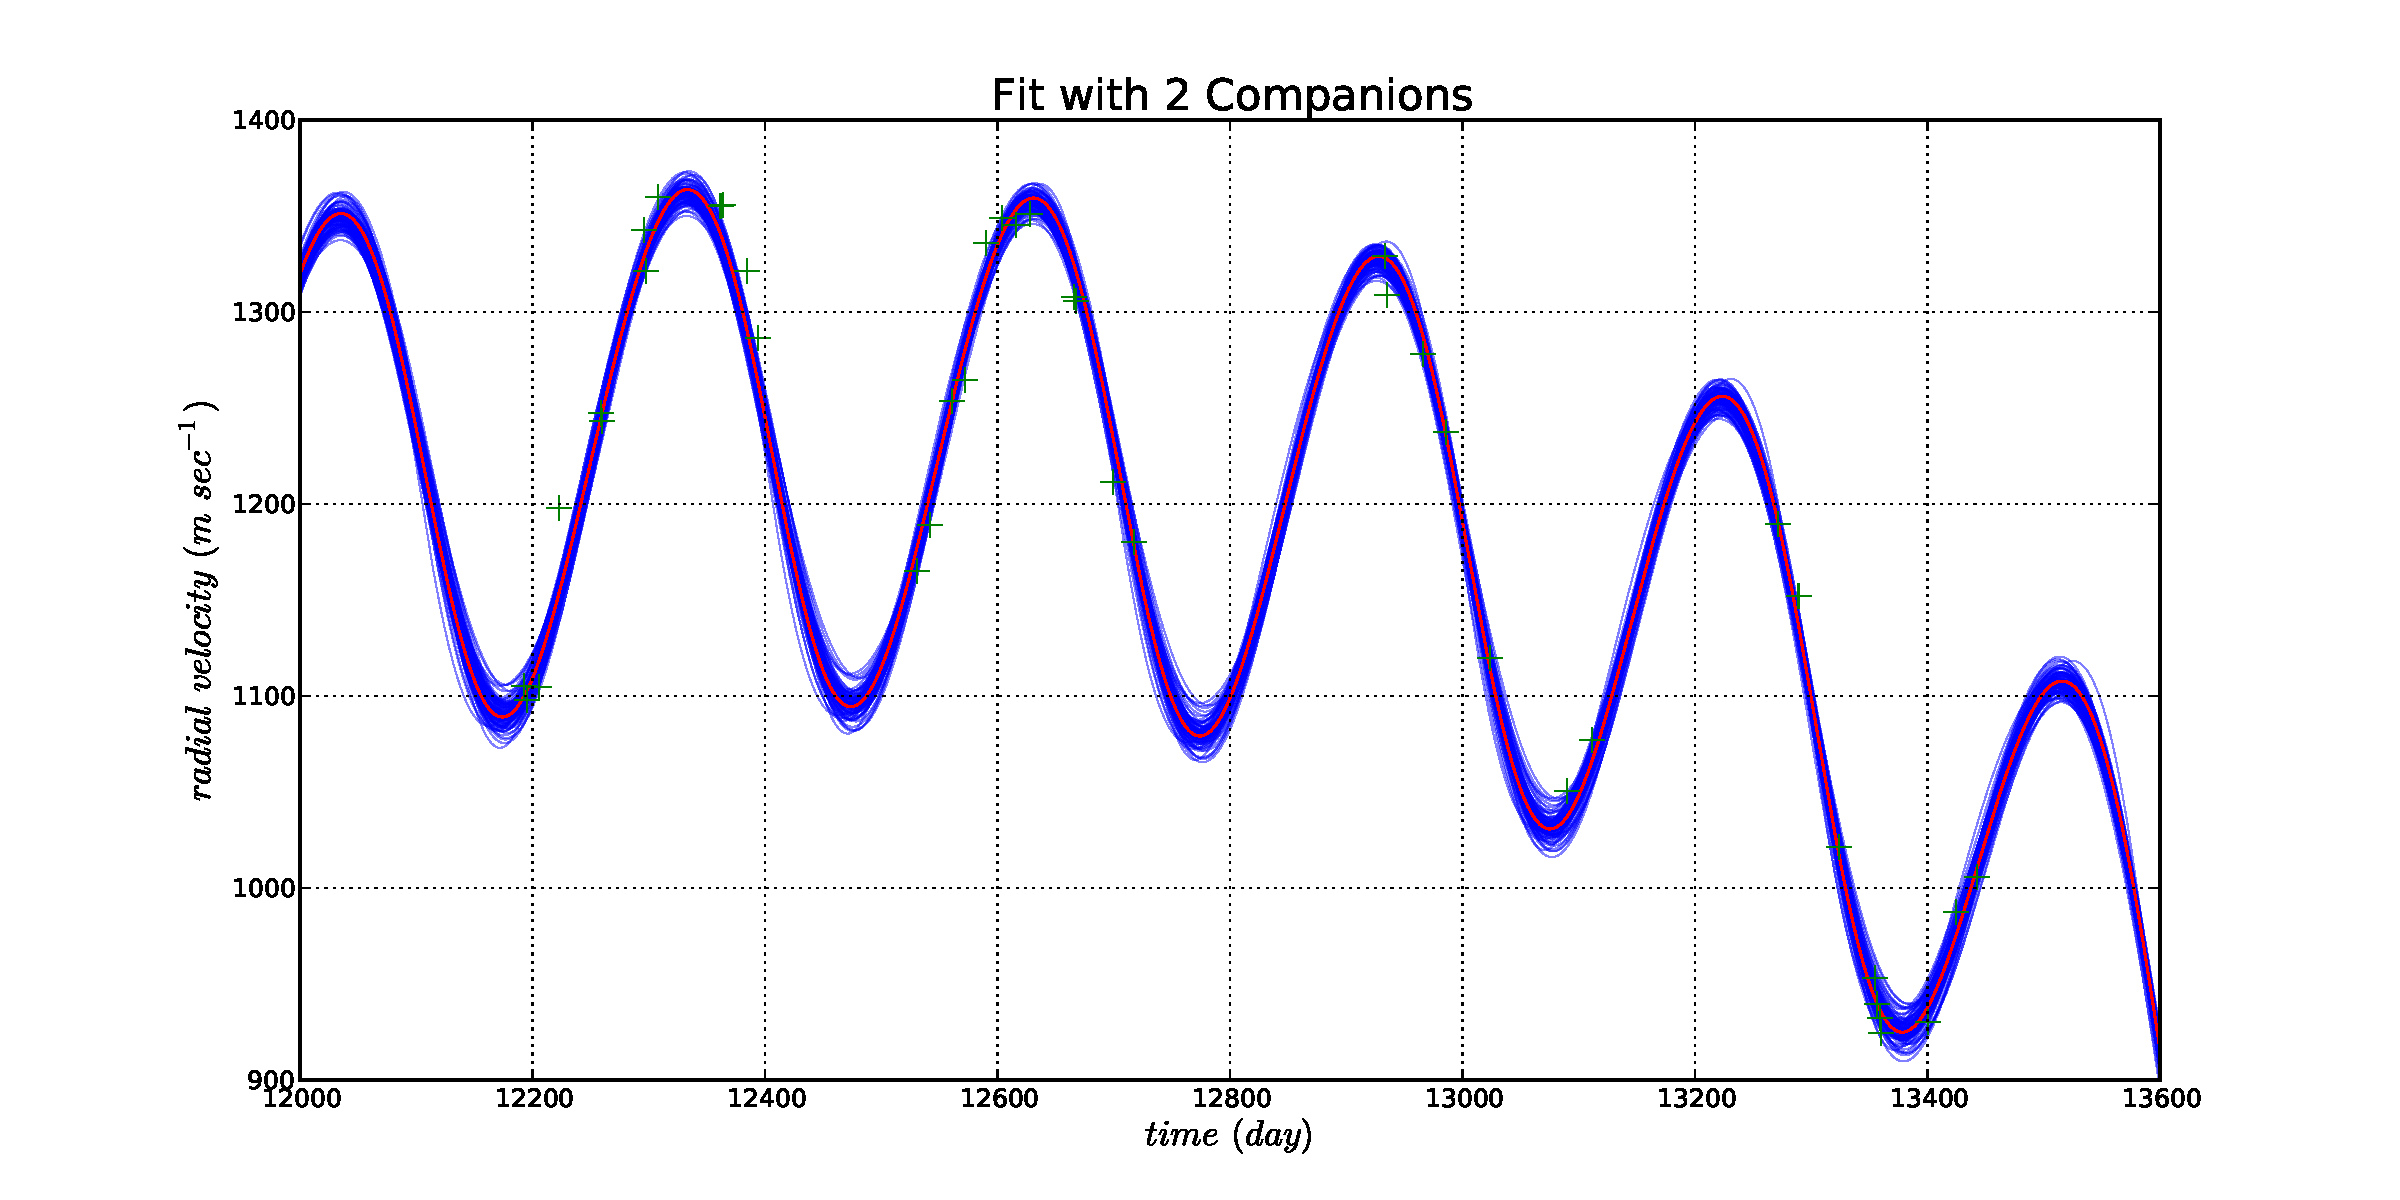
\includegraphics[width=0.99\linewidth]{fit_122_comp_2_small.pdf}\\
 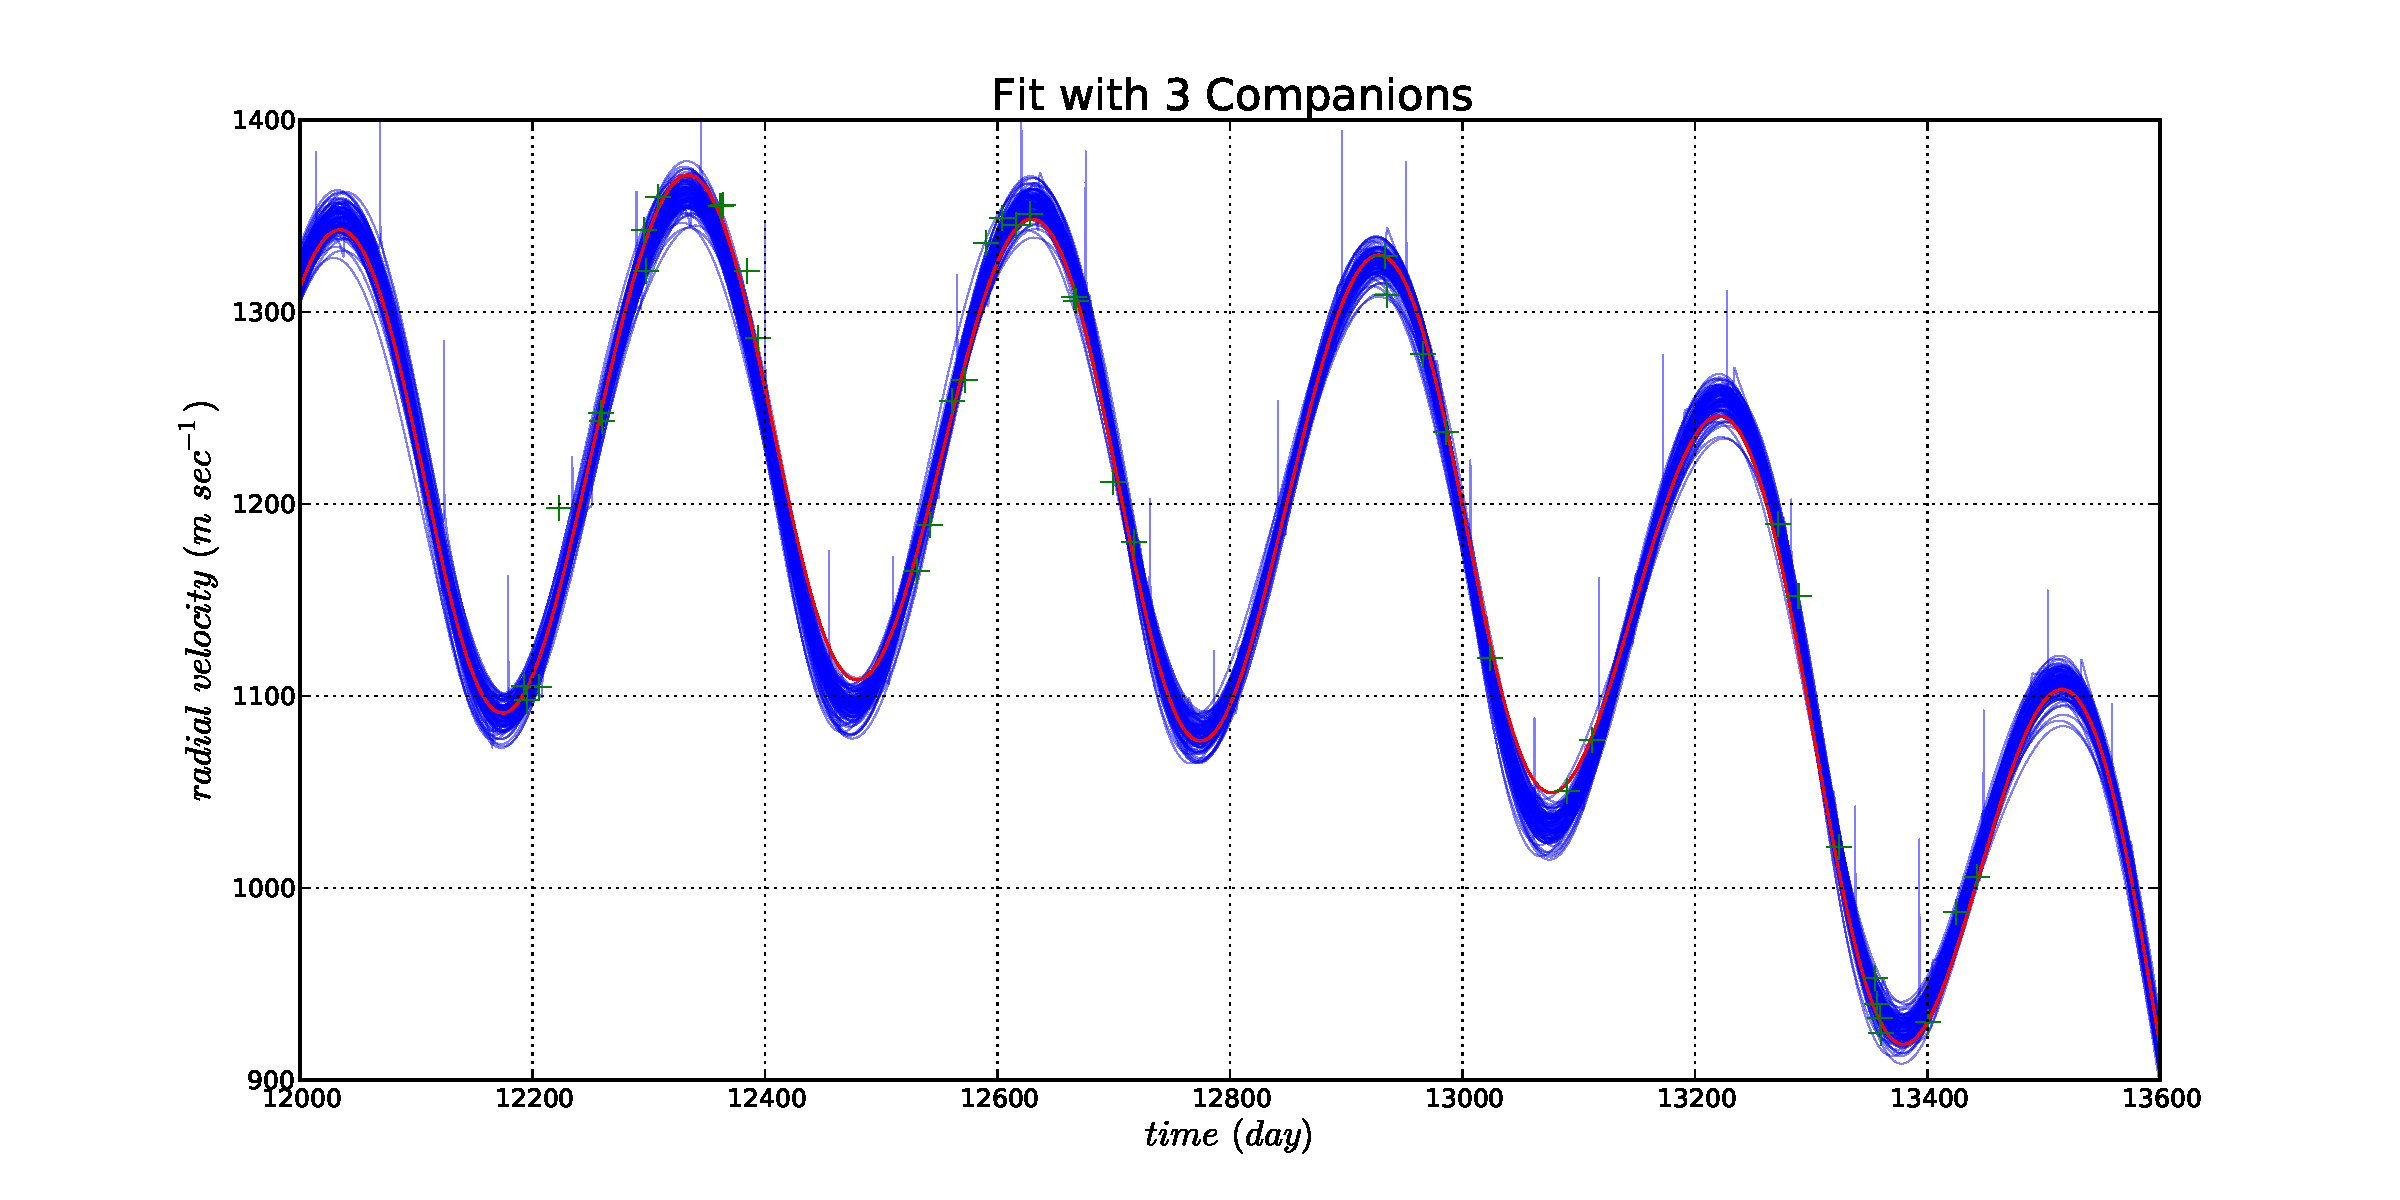
\includegraphics[width=0.99\linewidth]{fit_122_comp_3_small.pdf}
\caption{The 1st row shows the fit of 2-companion model zoomed in.  The 2nd row shows the fit of 3-companion model zoomed in. The \textcolor{red}{red curves} in the center indicate the optimal fits. The 3-companion fit is only slightly better than the 2-companion fit. Because the optimally-fit 'well' in the 3-companion fit is too shallow. Some of the 3-companion fits actually come from local minima. (In the figure, some fits are spiky which indicates over-fitting.)}
 \label{fig:fit-122-2-3-zoom}
\end{figure}

\end{document}
